\section{Resultados e Avaliação de Performance (Engenharia)}

A seção de Resultados subdivide-se em duas esferas de validação. Inicialmente, uma bateria de testes sob estresse estabelece os limites arquiteturais do motor Apache Druid, atestando a estabilidade da engenharia de \textit{hardware} frente a gargalos induzidos. Em seguida, a pesquisa transpõe o \textit{pipeline} estruturado para o mundo real, operando-o na simulação tática do cenário de crise climática e ambiental brasileira ao longo do ano de 2025.

\subsection{Volumetria Espacial e Eficiência de Compressão}

Antes de prosseguir com a análise de vazão computacional, a Tabela \ref{tab:volumetria} consolida a magnitude da infraestrutura analítica do SIRDA. Embora a camada analítica (OLAP) lide com um montante superior a 4 milhões de entidades, o peso total de armazenamento nos \textit{Historical Nodes} não ultrapassou a marca de 850 Megabytes físicos, distribuídos em 695 segmentos compactados.

\begin{table}[H]
    \centering
    \caption{Volumetria de Entidades no Apache Druid.}
    \label{tab:volumetria}
    \resizebox{\textwidth}{!}{%
    \begin{tabular}{llrr}
        \hline
        \textbf{Entidade Lógica} & \textbf{Tipo} & \textbf{Registros Aprox.} & \textbf{Função no Esquema} \\ \hline
        Fato Focos Incêndio & Fato & 3.335.198 & Coordenadas brutas INPE/NASA \\
        Fato Eventos Incêndio & Fato & 147.560 & Polígonos DBSCAN \\
        Hospitais (CNES) & Dimensão & 550.882 & Ativos de pressão humanitária \\
        Rodovias Federais (DNIT) & Dimensão & 14.255 & Logística e evacuação \\
        Subestações e Linhas (ONS) & Dimensão & 2.564 & Malha energética sistêmica \\
        Municípios Brasileiros \cite{brugz_geodata_2026} & Dimensão & 5.564 & Malha geopolítica e demográfica \\
        Terras Indígenas (FUNAI) & Dimensão & 650 & Polígonos de fronteira étnica \\ \hline
        \textbf{Total Analítico} & -- & \textbf{4.056.673} & \textbf{Alocados em $\sim$850 MB} \\ \hline
    \end{tabular}%
    }
\end{table}

Essa eficiência de compactação colunar atesta na prática as escolhas arquiteturais do \textit{Esquema Constelação} atrelado ao motor Druid. Ao delegar o peso geométrico complexo integralmente às Tabelas de Dimensão e operá-las via \textit{Lookups} globais, a arquitetura isola o crescimento massivo das anomalias térmicas, viabilizando as métricas de baixíssima latência que serão discutidas nas baterias de testes subsequentes.

\subsection{Avaliação Preliminar do Motor Analítico (Março/2026)}

Um estudo preliminar (março de 2026) avaliou o desempenho bruto do Apache Druid sobre \textasciitilde{}3,1 milhões de registros do INPE. Naquela etapa inicial do projeto, a arquitetura Silver ainda não havia sido desenvolvida. Portanto, o cenário operava exclusivamente com filtros tabulares simples sobre a tabela fato crua, sem o gargalo matemático das intersecções espaciais complexas (GeoJSON).

O experimento submeteu 6 \textit{queries} de referência a diferentes alocações de CPU (2, 4 e 6 núcleos) em dois cenários opostos: estado bruto de ingestão (fragmentado em 6.518 \textit{Tiny Segments}) e estado compactado (granularidade \texttt{YEAR}).

A Figura \ref{fig:abismo_desempenho} sintetiza o impacto estrutural. No estado fragmentado, o sistema atingiu um teto de I/O em \textasciitilde{}1.624ms mesmo com 6 núcleos, evidenciando a Lei de Amdahl perante o \textit{overhead} de 6.518 \textit{file handles}. Em contraste, a simples compactação despencou a latência média para \textasciitilde{}55ms. Mantendo o mesmo hardware, a aceleração chegou a quase 39 vezes no cenário de 4 núcleos. Com o disco organizado, todas as consultas passaram a responder em sub-100ms utilizando apenas 2 núcleos (Figura \ref{fig:barras_compactado}).

\begin{figure}[H]
    \centering
    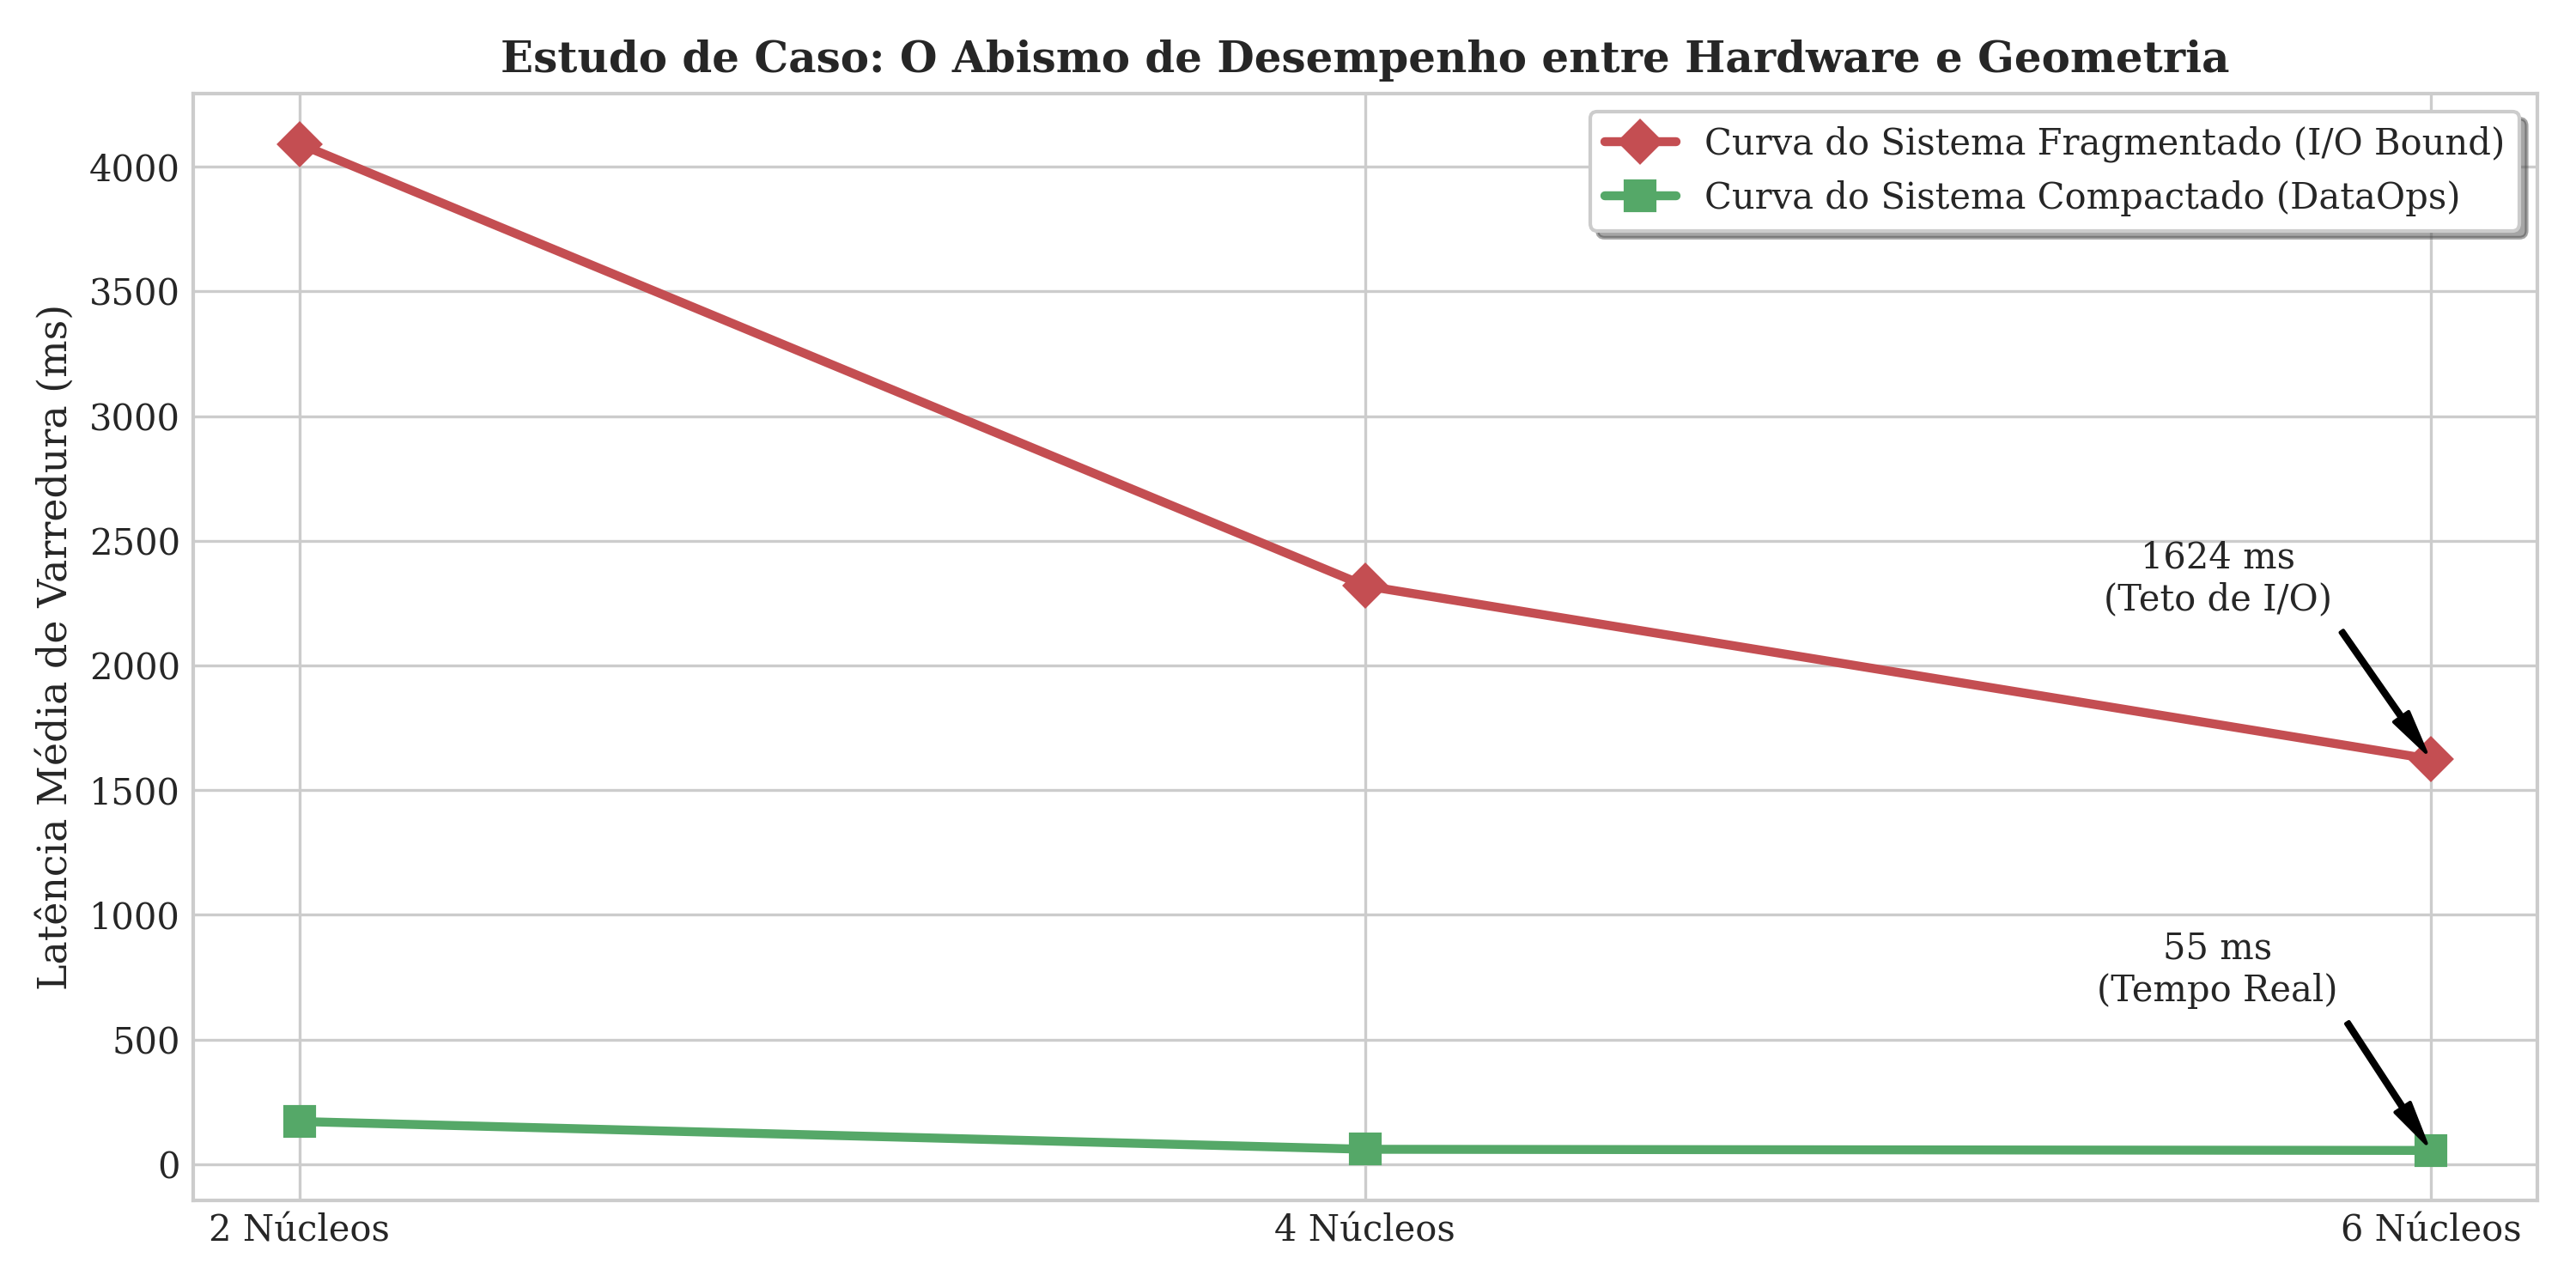
\includegraphics[width=0.85\textwidth]{materiais_apoio/figures/benchmark_preliminar/r3_comparativo_latencia_geral.png}
    \caption{Comparativo de Desempenho: Dados Fragmentados vs. Compactados.}
    \label{fig:abismo_desempenho}
\end{figure}

A Tabela \ref{tab:fator_dataops} quantifica a magnitude dessa otimização. A intervenção algorítmica revelou-se sistematicamente superior à infraestrutura física: o sistema estrangulado a 2 núcleos lendo a base compactada (171ms) foi, na prática, \textbf{\textasciitilde{}9,5 vezes} mais rápido do que o hospedeiro em potência máxima (6 núcleos) tentando processar o caos estrutural (1.624ms).

\begin{table}[H]
    \centering
    \footnotesize
    \caption{Redução de Latência Relativa por Alocação de CPU.}
    \label{tab:fator_dataops}
    \begin{tabular}{lccc}
        \toprule
        \textbf{Hardware} & \textbf{Cold Start (Frag.)} & \textbf{Cold Start (Comp.)} & \textbf{Aceleração} \\
        \midrule
        2 Núcleos & 4.092 ms & 171 ms & 23,9$\times$ \\
        4 Núcleos & 2.320 ms & 60 ms  & 38,8$\times$ \\
        6 Núcleos & 1.624 ms & 55 ms  & 29,4$\times$ \\
        \bottomrule
    \end{tabular}
\end{table}

\begin{figure}[H]
    \centering
    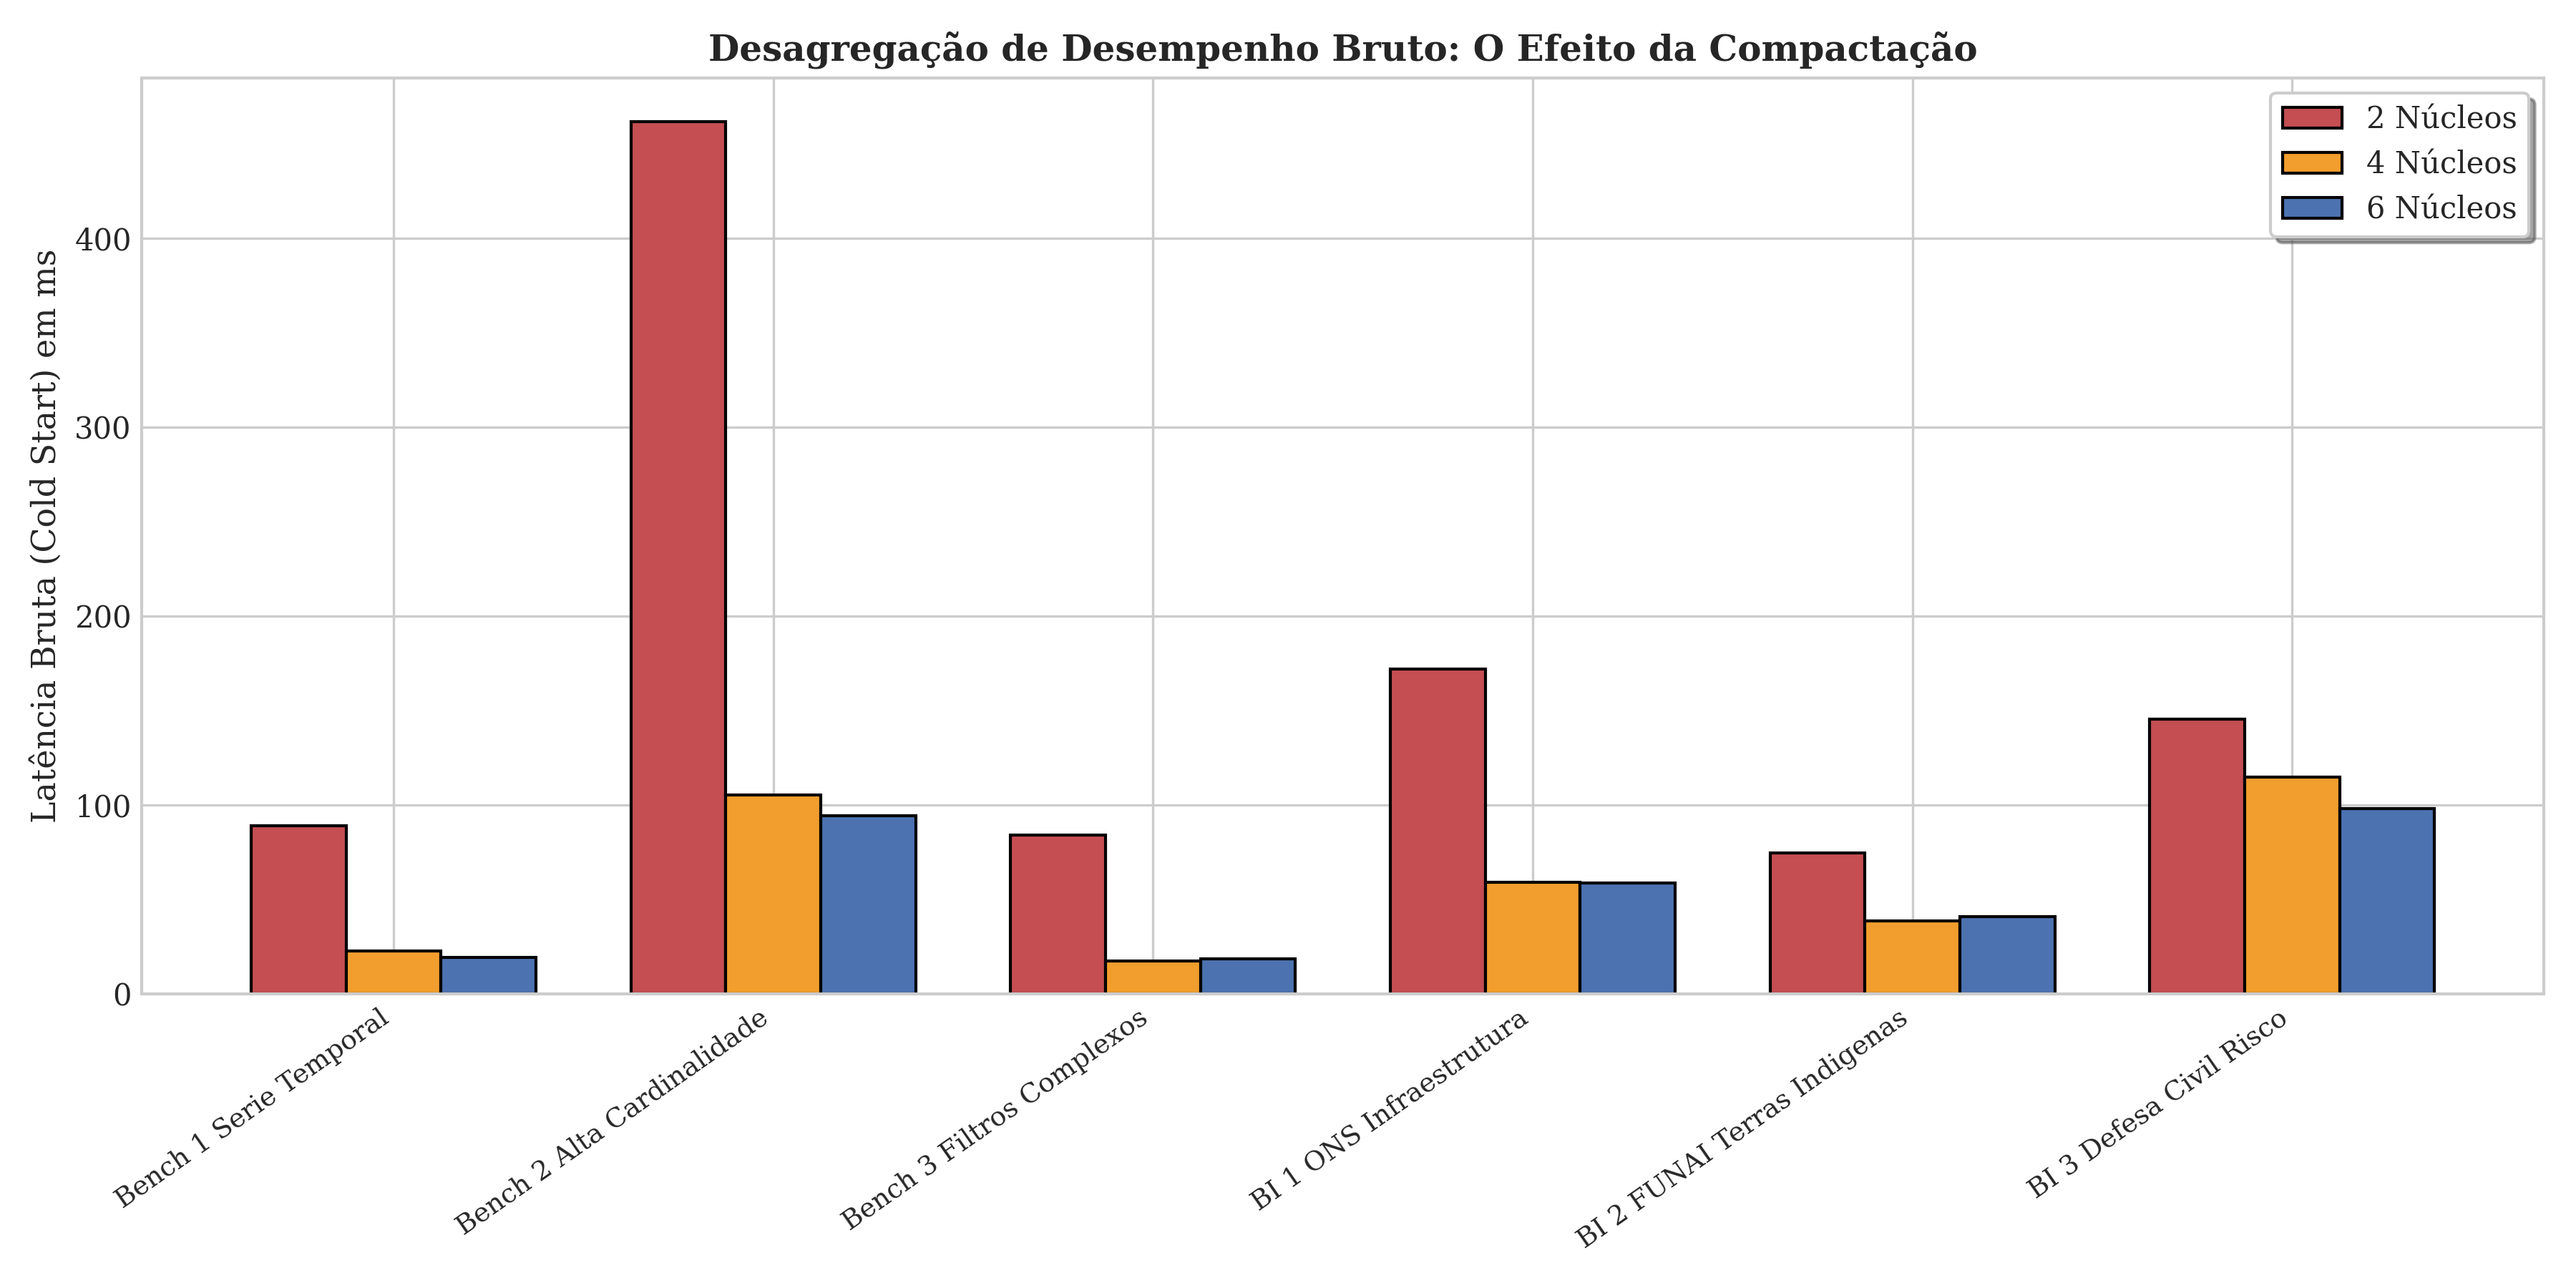
\includegraphics[width=0.85\textwidth]{materiais_apoio/figures/benchmark_preliminar/r2_latencia_por_cpu_compactado.png}
    \caption{Latência por Domínio de Consulta após Compactação (Março/2026).}
    \label{fig:barras_compactado}
\end{figure}

\subsection{Matriz de Capacidade e Saturação (Throughput)}

Embora a arquitetura básica exija escasso poder computacional (sub-100ms com 2 núcleos), a topologia \textit{Medallion} introduz alta complexidade matemática. O carregamento estrito de volumetrias da camada \textit{Silver} (e.g., polígonos GeoJSON de Terras Indígenas) desloca violentamente o gargalo sistêmico do I/O de disco para a CPU e Memória (\textit{Heap} da JVM). Para validar a resiliência estrutural a esse cenário logístico severo, executou-se a matriz de capacidade concorrente.

A avaliação atestou que a renderização de mapas analíticos sob a arquitetura empregada é primariamente \textit{CPU-Bound}. O cenário \textbf{Baseline (1.0 CPU)} apresentou degradação de desempenho logo no primeiro operador, estagnando em \textbf{0,89 QPS} com falha em 42,7\% das requisições (\textit{Timeouts}). Isso atesta que um núcleo solitário não sustenta a alta carga de alocação de memória exigida pelos \textit{Lookups} dimensionais (que transferem as volumosas matrizes GeoJSON, previamente cruzadas na camada Silver pelo Python, para o \textit{Heap} do Druid).

Em contrapartida, a alocação expandida no cenário \textbf{Query Heavy (2.0 CPU)} demonstrou resiliência operacional. O sistema escalou a vazão (\textit{Throughput}) de forma constante, suportando até 16 \textit{threads} simultâneas e formando um platô sustentável na marca de \textbf{\textasciitilde{}2,0 QPS}. Nesse estado resiliente, novas conexões aguardam em fila, mas são integralmente entregues sem geração de \textit{Timeouts HTTP 500} (0\% de erro).

Nota-se, contudo, a presença eventual de \textit{outliers} negativos na curvatura de vazão linear. Em pontos específicos da escalada da carga, o sistema sofreu quedas abruptas de vazão em janelas milissegundares. Levanta-se a forte hipótese técnica de que este comportamento anômalo remeta a pausas prolongadas de \textit{Garbage Collection} (GC \textit{Stop-The-World}) e a eventos de \textit{Thread Contention}, embora essa suposição exigisse medições com \textit{profilers} ativos na JVM para constatação isolada.

\begin{figure}[H]
    \centering
    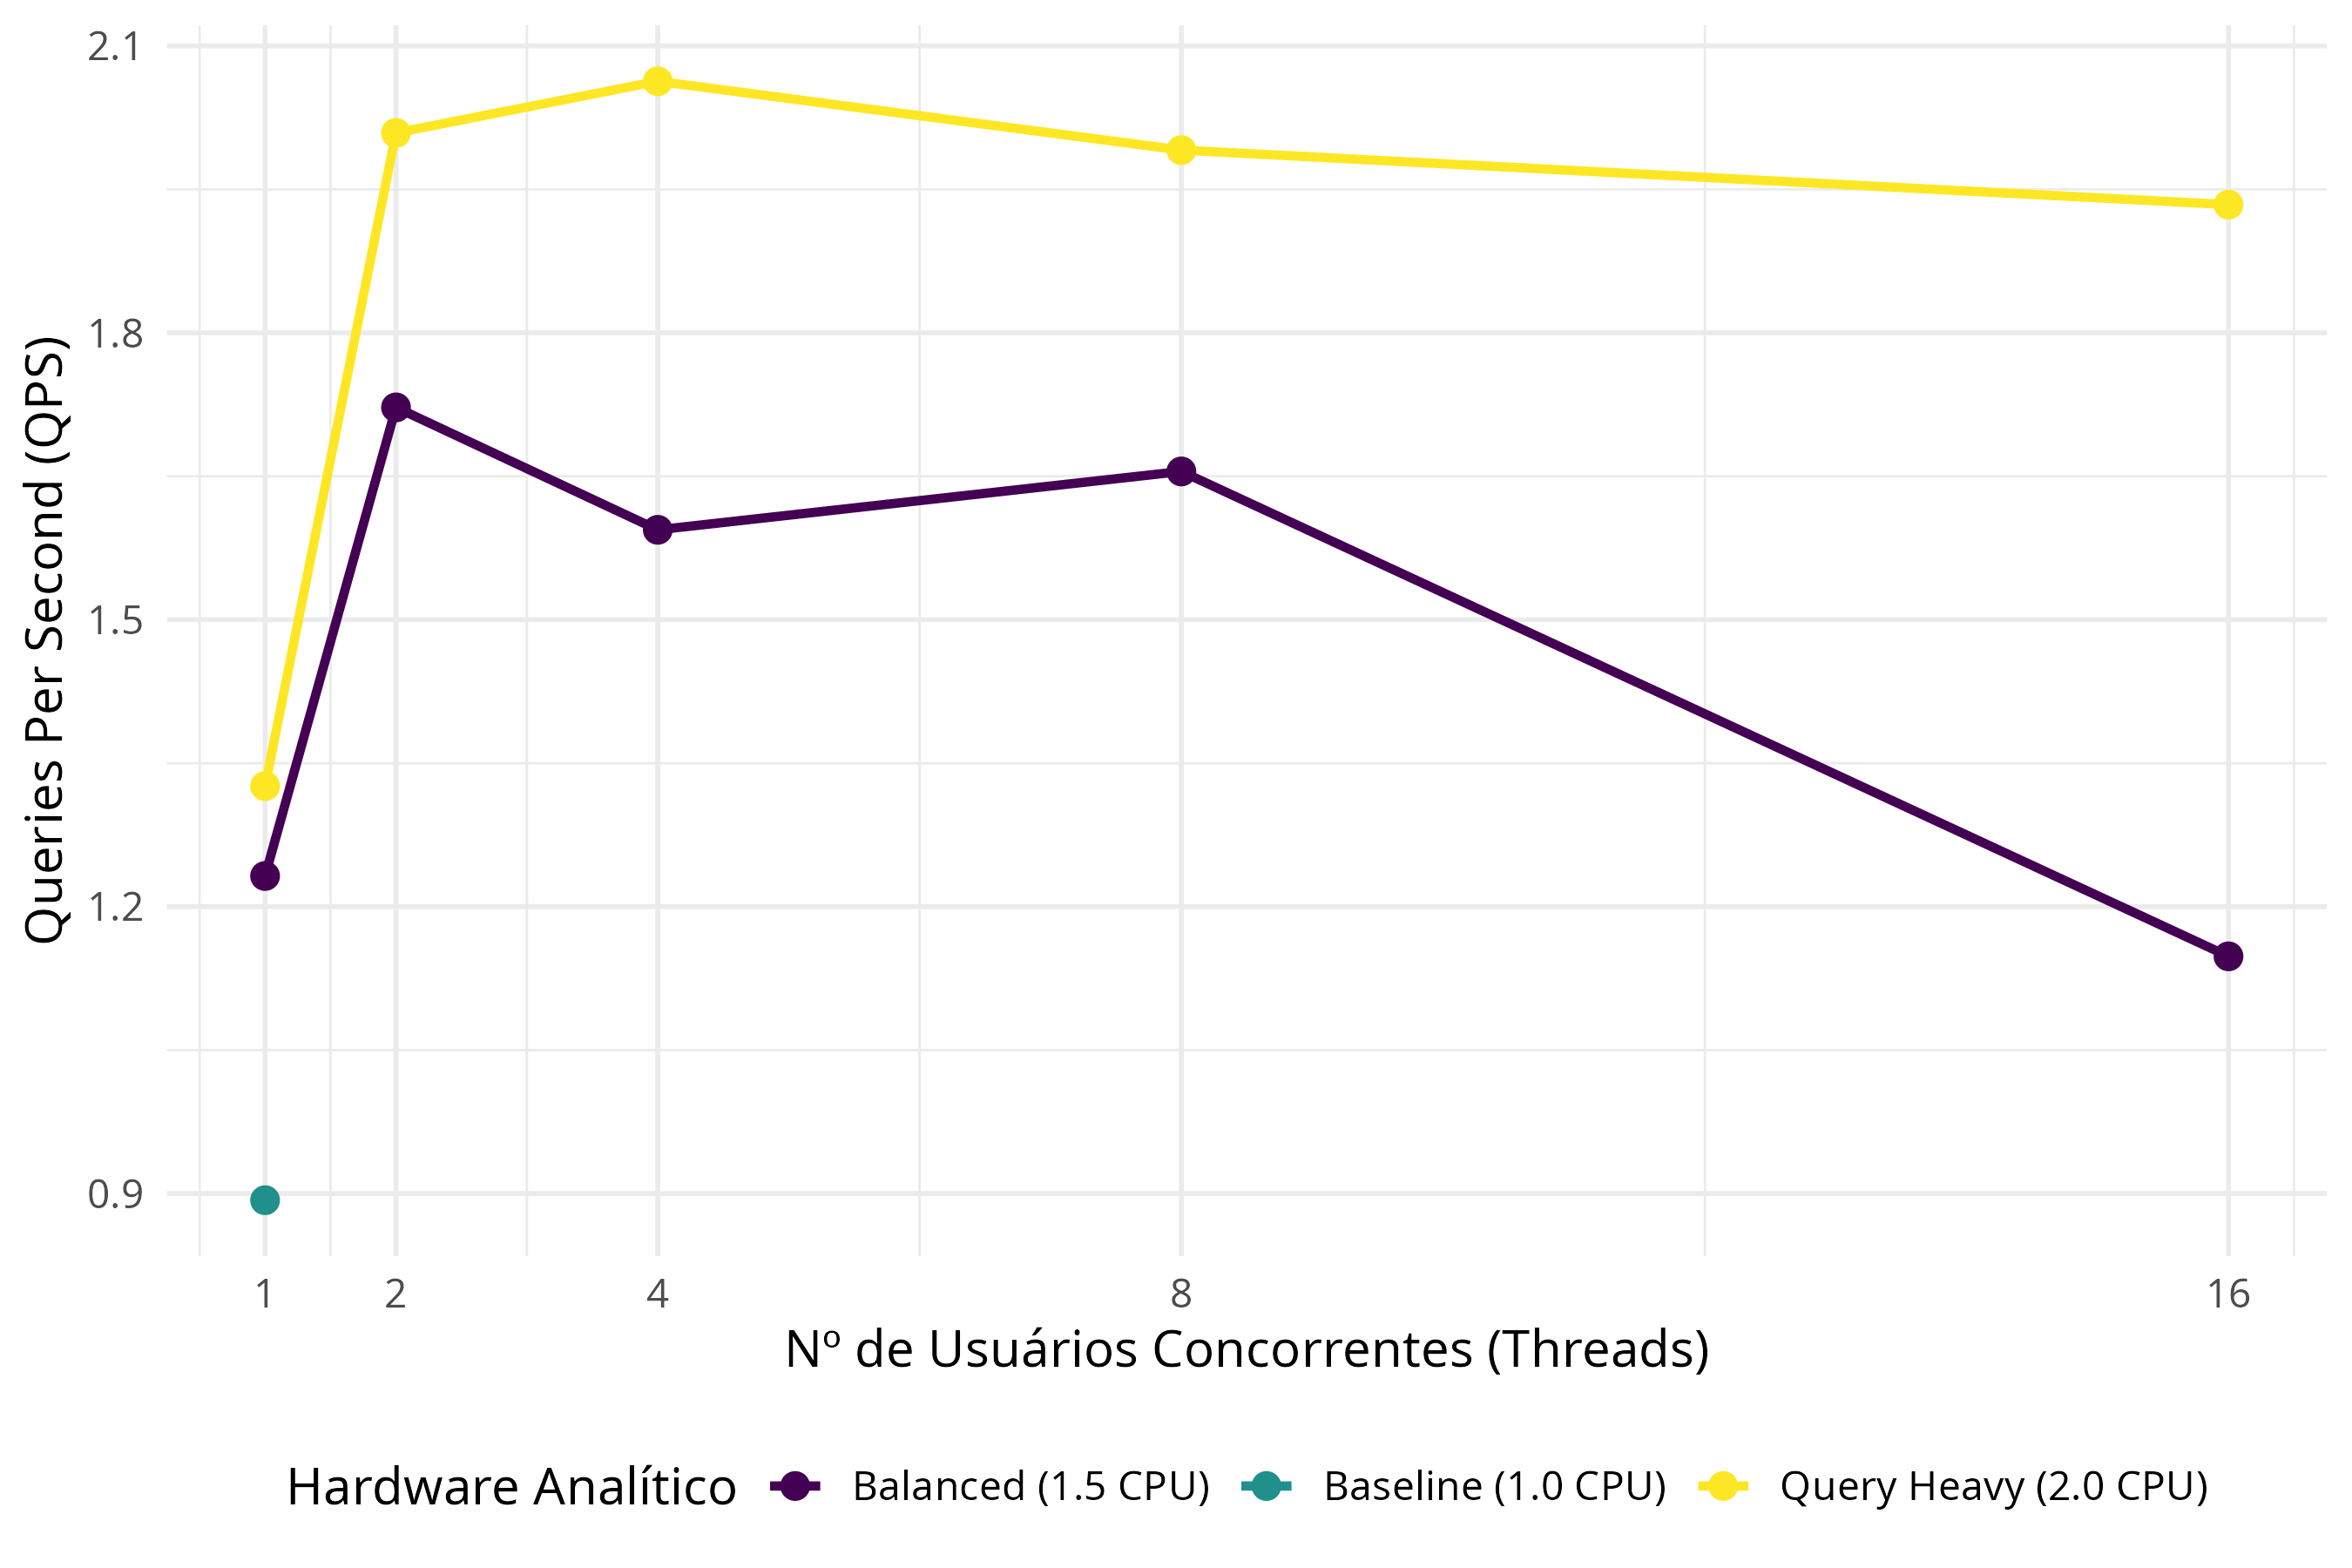
\includegraphics[width=0.8\textwidth]{analise_R/plots/qps_saturation_new.png}
    \caption{Vazão Analítica (QPS) por Perfil de Escalabilidade.}
    \label{fig:qps_saturation}
\end{figure}

\subsection{Explosão de Latência e Percentil 95 (P95)}

Conforme demonstrado estatisticamente, no cenário \textit{Baseline} a latência e o volume de falhas descontrolaram-se já no primeiro operador em rede. Em contraste, o cenário \textit{Query Heavy} absorveu o impacto geométrico sem gerar interrupções, contendo a latência P95 na faixa aceitável de \textbf{\textasciitilde{}2,8 segundos} (com 2 operadores) até o limiar de \textbf{\textasciitilde{}8,2 segundos} sob o estresse de 8 operadores processando agregações massivas simultaneamente.

Contudo, fora da curva de 95\% (\textit{outliers}), registraram-se picos de latência. Esses engasgos ocorrem quando cruzamentos espaciais densos (e.g., sobreposição espacial em Terras Indígenas) esgotam a memória \textit{Heap} da JVM e os \textit{Merge Buffers}, forçando pausas prolongadas de \textit{Garbage Collection} (GC). Ressalta-se que tais anomalias foram induzidas por \textit{queries} puramente de estresse (sem amarras temporais). Na operação real do SIRDA, filtros de temporalidade (ex: janela crítica de 7 dias) impedem que um pacote GeoJSON dessa magnitude congestione a memória em uma única requisição.

\begin{figure}[H]
    \centering
    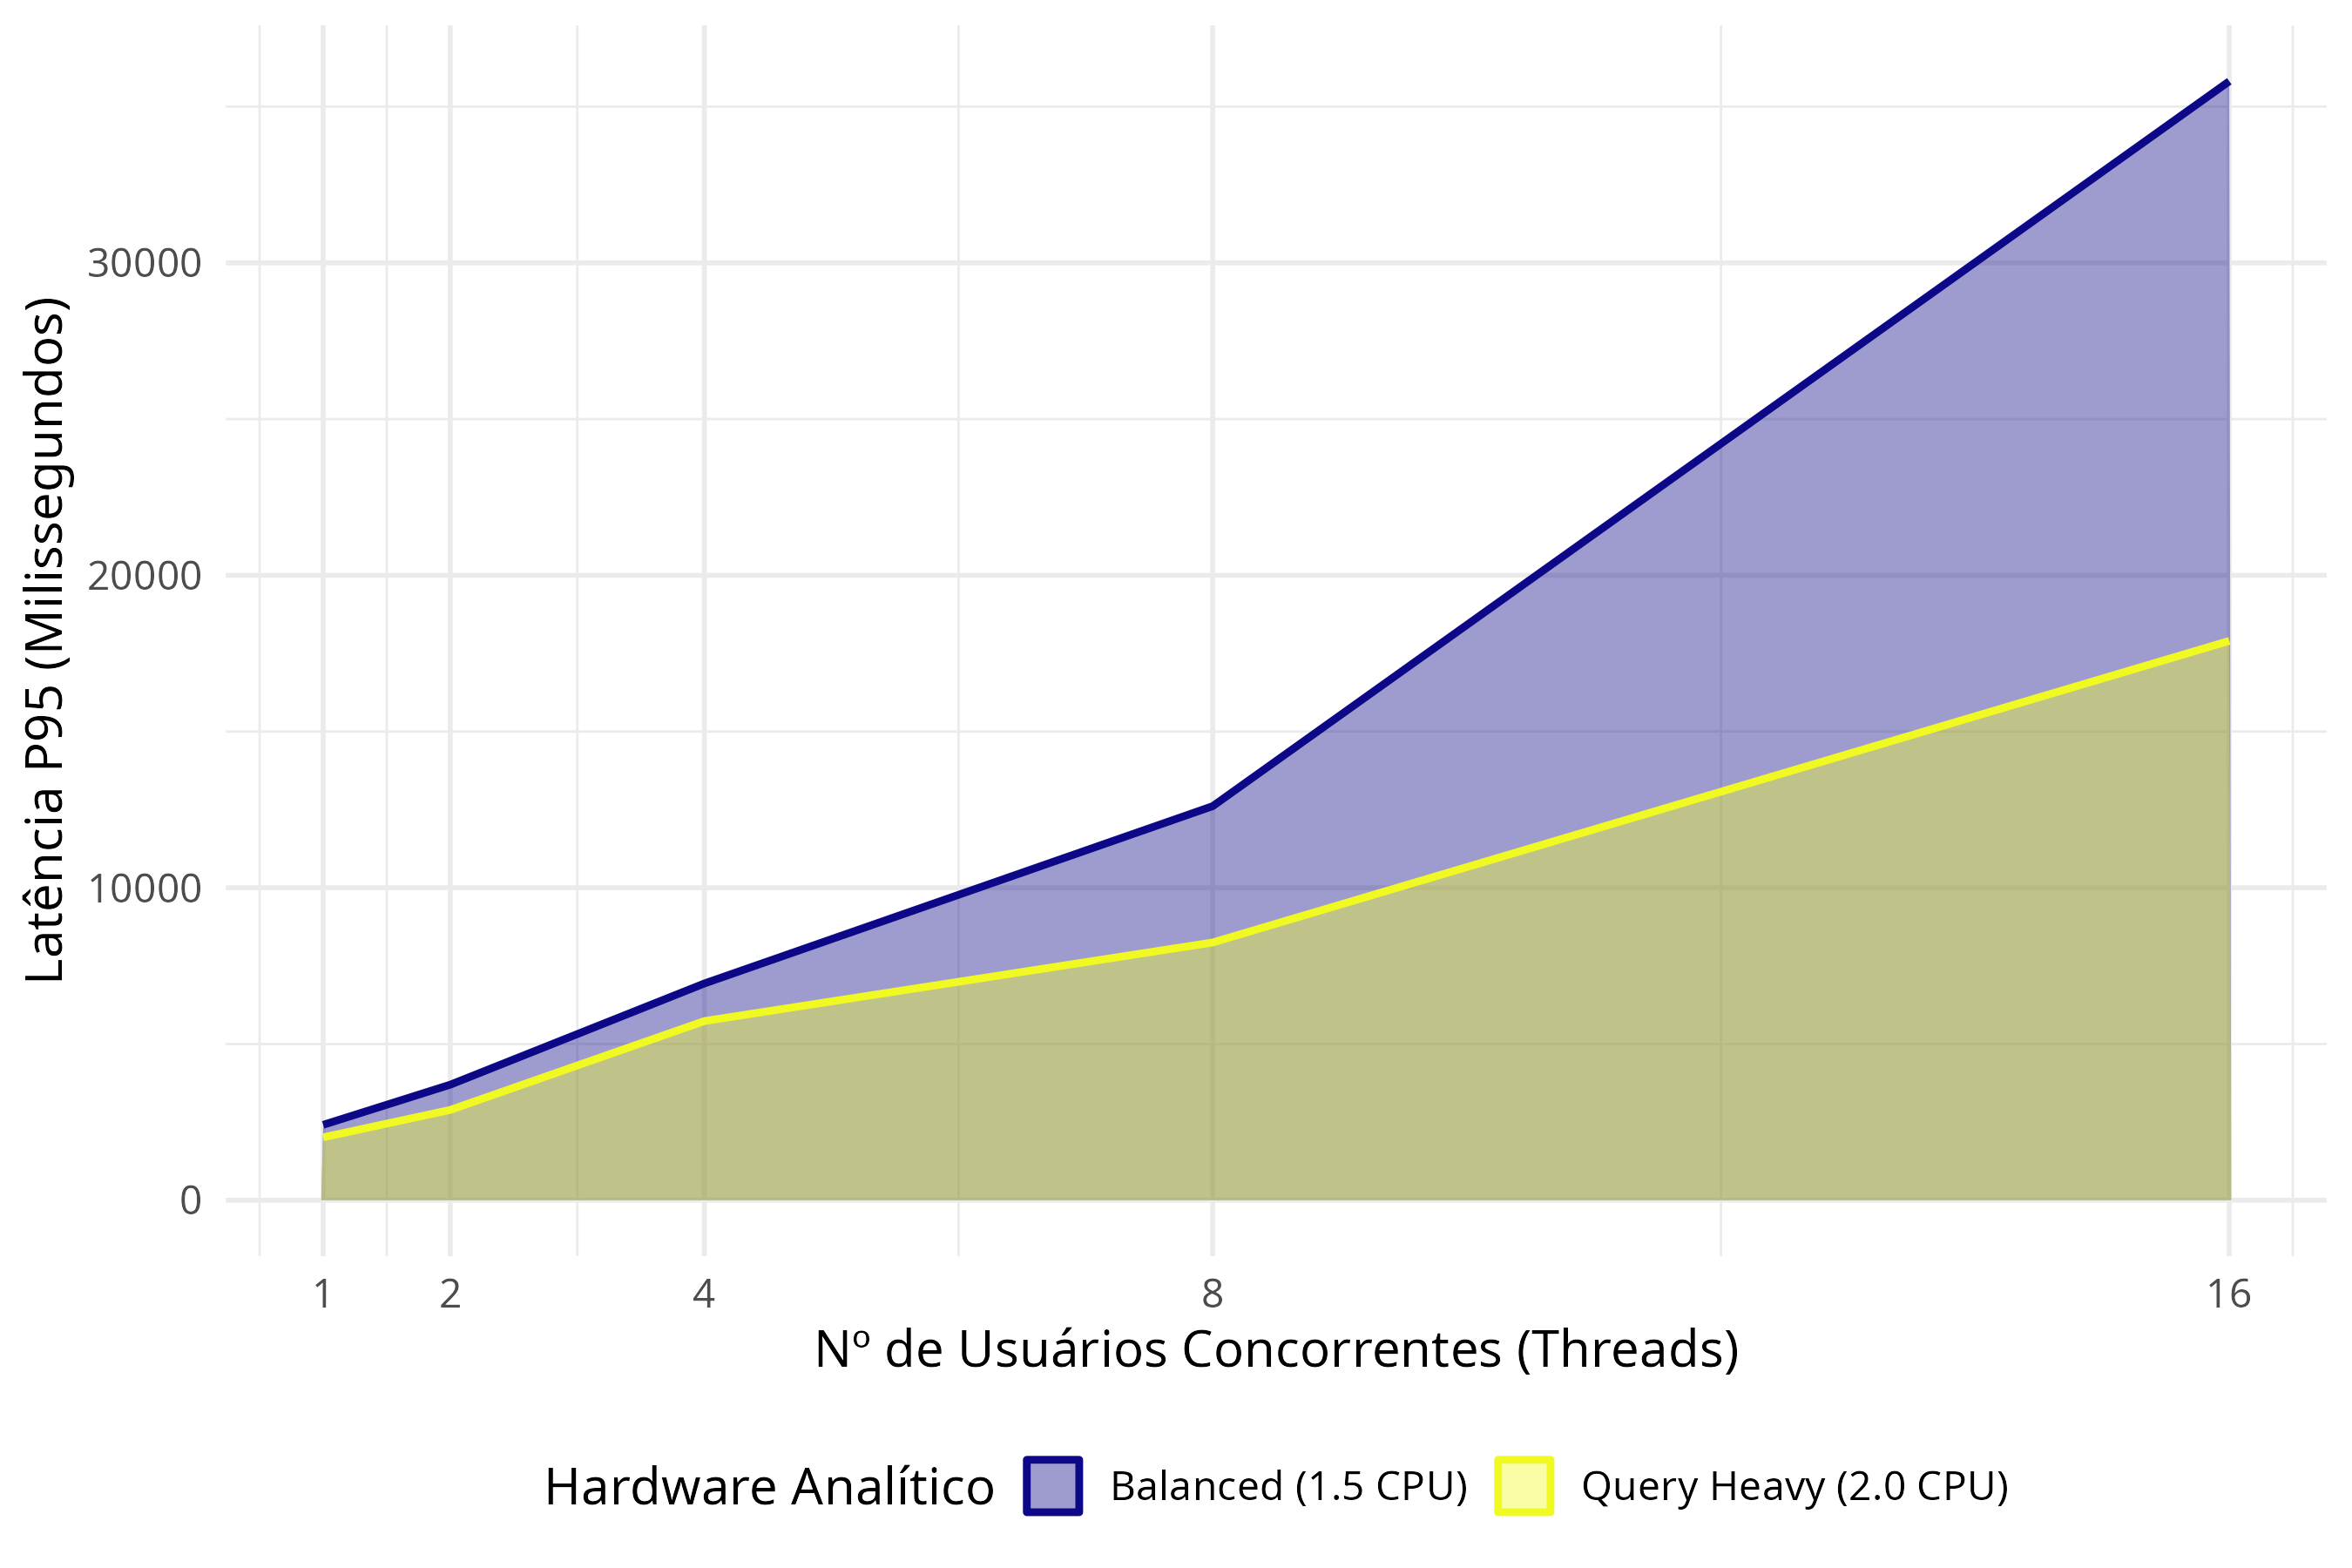
\includegraphics[width=0.8\textwidth]{analise_R/plots/p95_latency_new.png}
    \caption{Degradação de Latência (P95) durante Escalonamento.}
    \label{fig:p95_latency}
\end{figure}

\subsection{Eficiência do Mecanismo de Cache de Memória}

No contexto operacional da plataforma SIRDA, painéis gerenciais (\textit{Dashboards}) promovem uma forte redundância de consultas similares por diferentes operadores. O mecanismo nativo de intercepção (\textit{Broker Query Cache}) provou atuar mitigando a debilidade da restrição de processamento de núcleo.

Pela ótica da escala logarítmica representada, as requisições puras ao disco e aos segmentos de dados (\textit{Cold Start}) operam em densidades predominantemente acomodadas acima de $10^3$ (1.000 a 10.000 milissegundos). Por sua vez, o acerto de memória (\textit{Warm Start}) reduz drasticamente a latência para faixas abaixo de $10^2$ (sub-100 milissegundos), garantindo que metade da atividade analítica pesada seja entregue numa magnitude de quase tempo real e economizando leituras nos índices colunares subjacentes (\textit{Bitmap Indexes}).

A base matemática exibiu extensões esguias persistentes no violino de aquecimento (caudas longas no cenário \textit{Warm}), atestando instantes em que requisições repetidas demoraram o mesmo ou até mais tempo que requisições originais em disco. A hipótese analítica primária para este fenômeno de \textit{outliers} recai sobre a ocorrência de \textit{Cache Eviction} sistêmico. Sob carga frenética e concorrente, postula-se que o vetor local de memória do \textit{Broker} lota precocemente de dados variados, sendo forçado a "despejar" (remover) painéis outrora armazenados.

\begin{figure}[H]
    \centering
    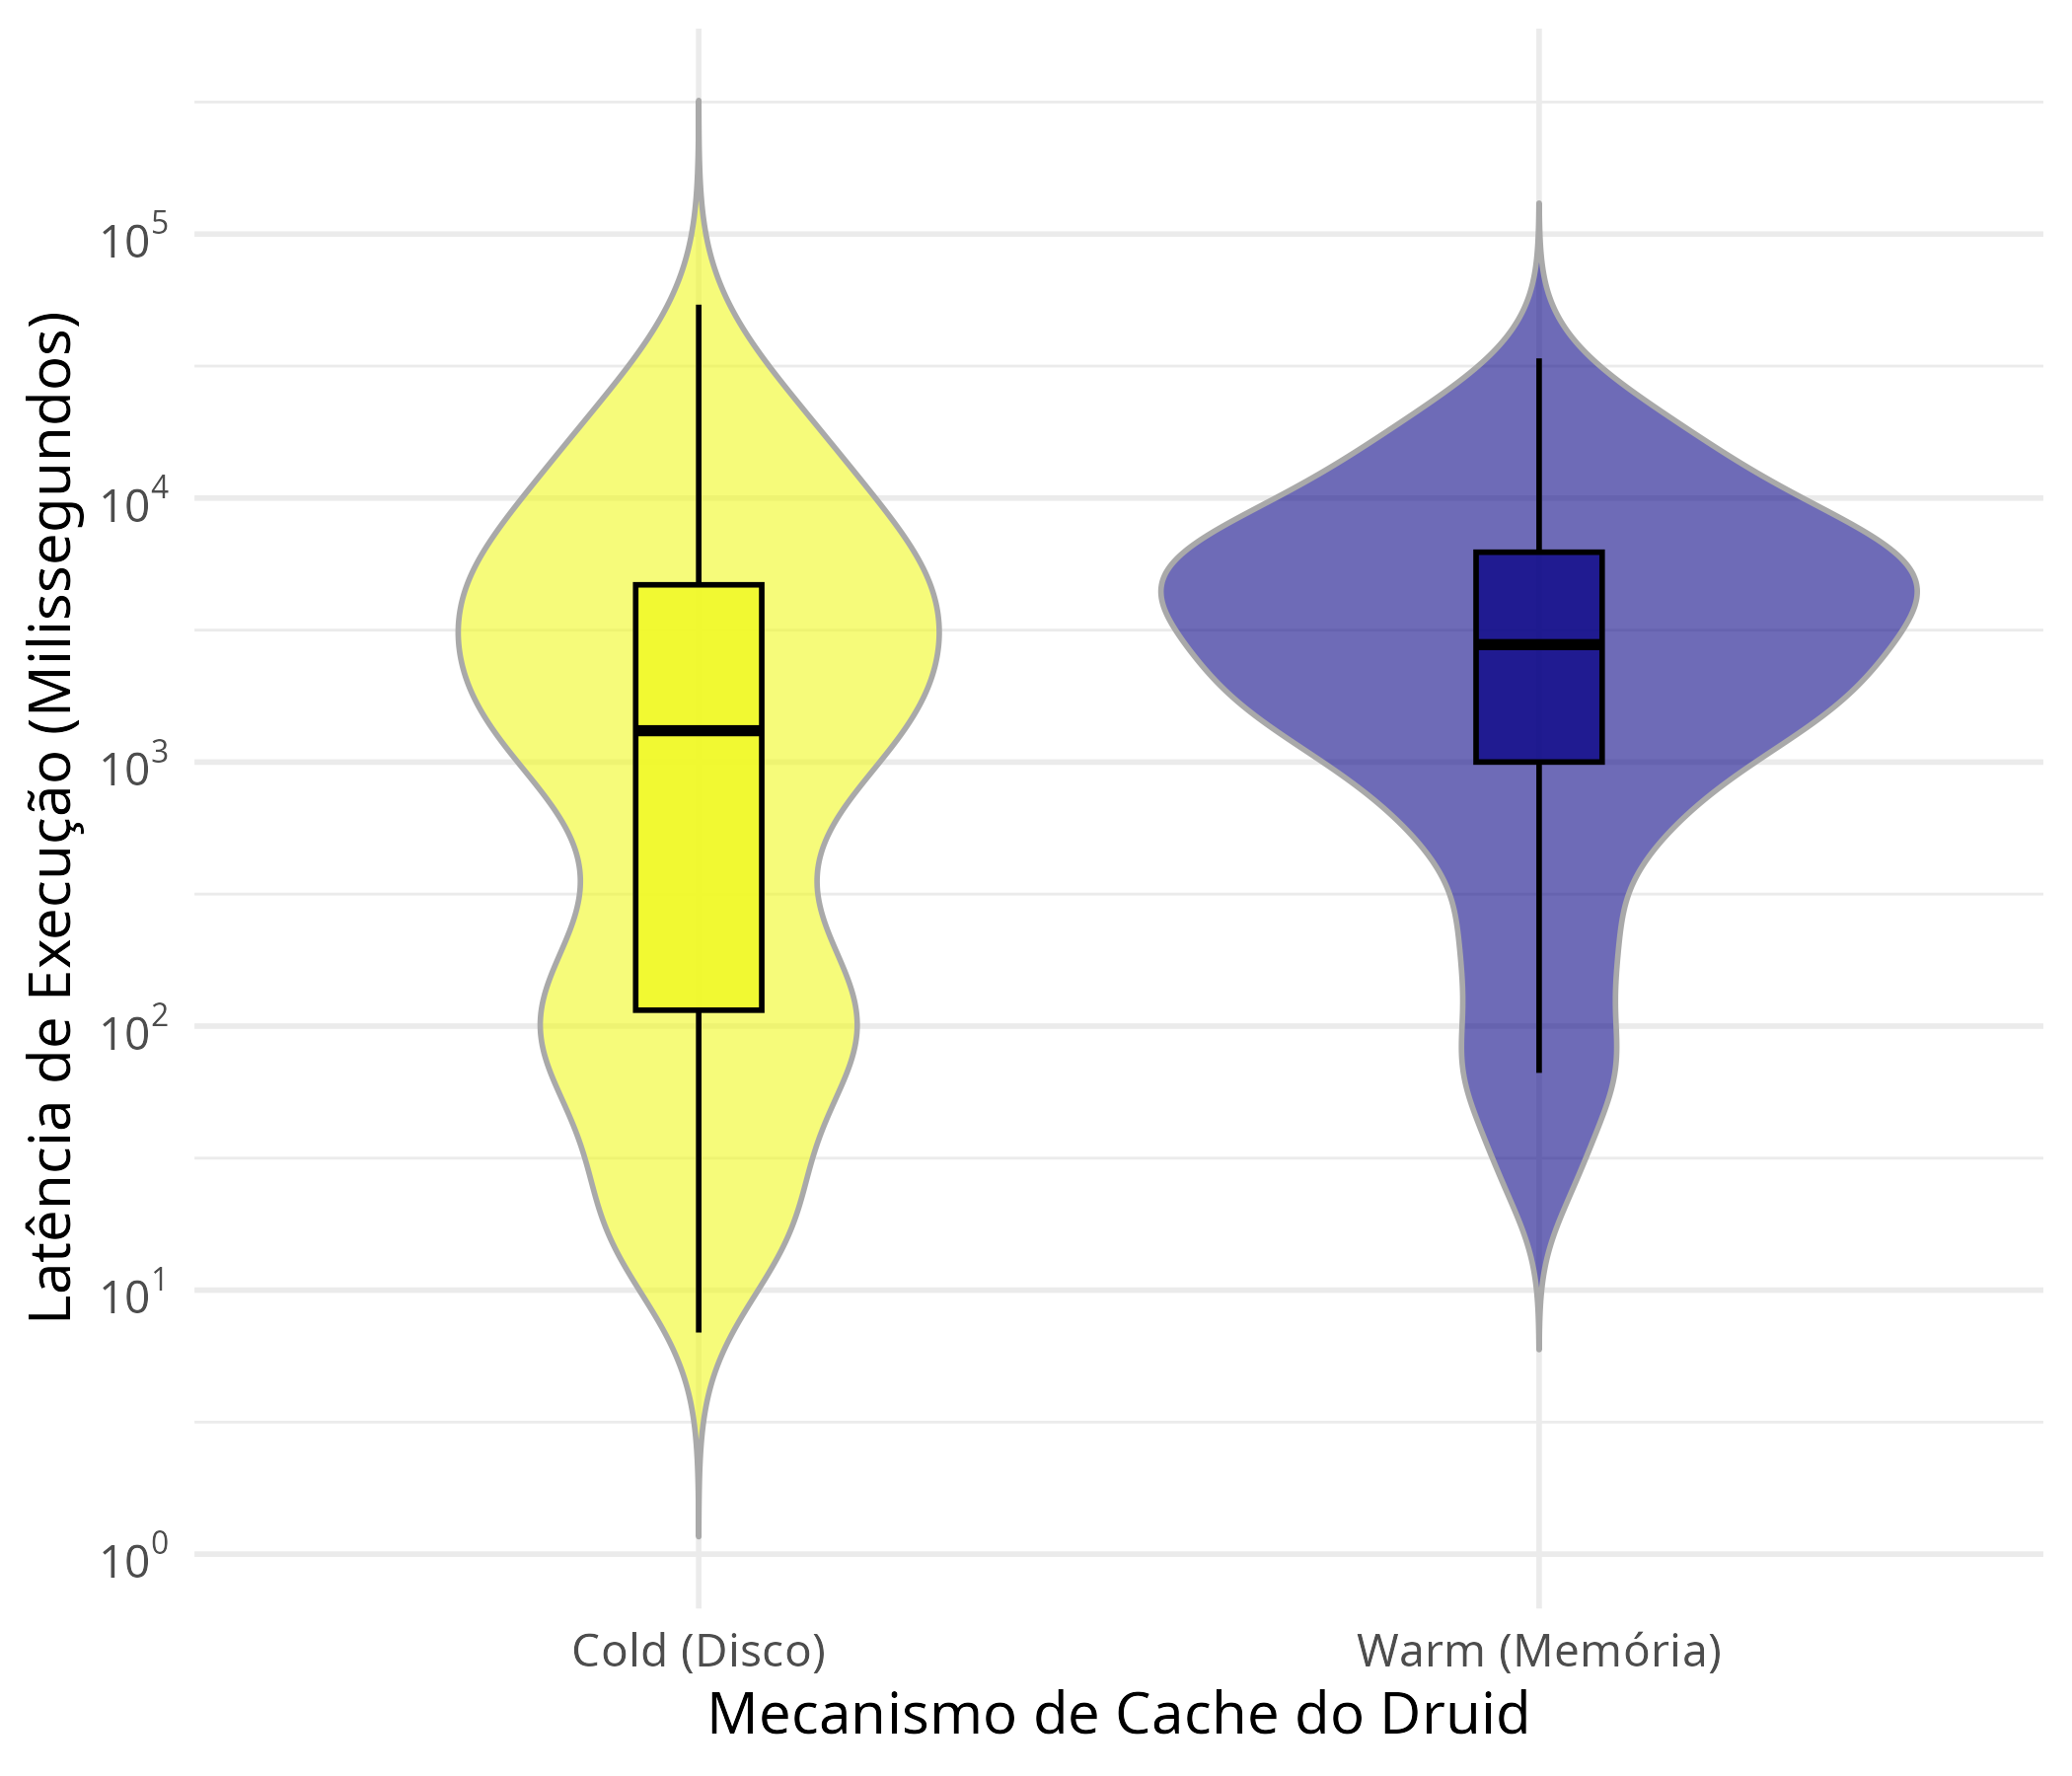
\includegraphics[width=0.8\textwidth]{analise_R/plots/cache_violin_new.png}
    \caption{Distribuição de Latência: Cache vs. Leitura Nativa.}
    \label{fig:cache_efficiency}
\end{figure}

\subsection{Consumo Físico de Contêineres e Esgotamento (Memory Footprint)}

A série temporal corrobora a estabilidade dos nós conteinerizados perante o limite estrito do \textit{Cgroup} (Docker), demonstrando teto rígido (inferior a 90\%) e atestando a ausência de vazamento de memória (\textit{Memory Leak}). O motor de varredura (\textit{Historical}) acomoda-se em platôs seguros (70\%-80\%) durante as rajadas de carga.

De maneira análoga, o contêiner integrador (\textit{Broker}) exibe um comportamento resiliente, evidenciando que grandes cargas cartográficas em memória (GeoJSON) são velozmente serializadas, com espaço recuperado pelas rotinas de limpeza da JVM (\textit{Garbage Collection}). Sem o registro de falhas por esgotamento (\textit{OOM Killed}), conclui-se que o verdadeiro gargalo analítico da plataforma reside no processamento matemático espacial (restrição de vCPU), e não na escassez de RAM.

\begin{figure}[H]
    \centering
    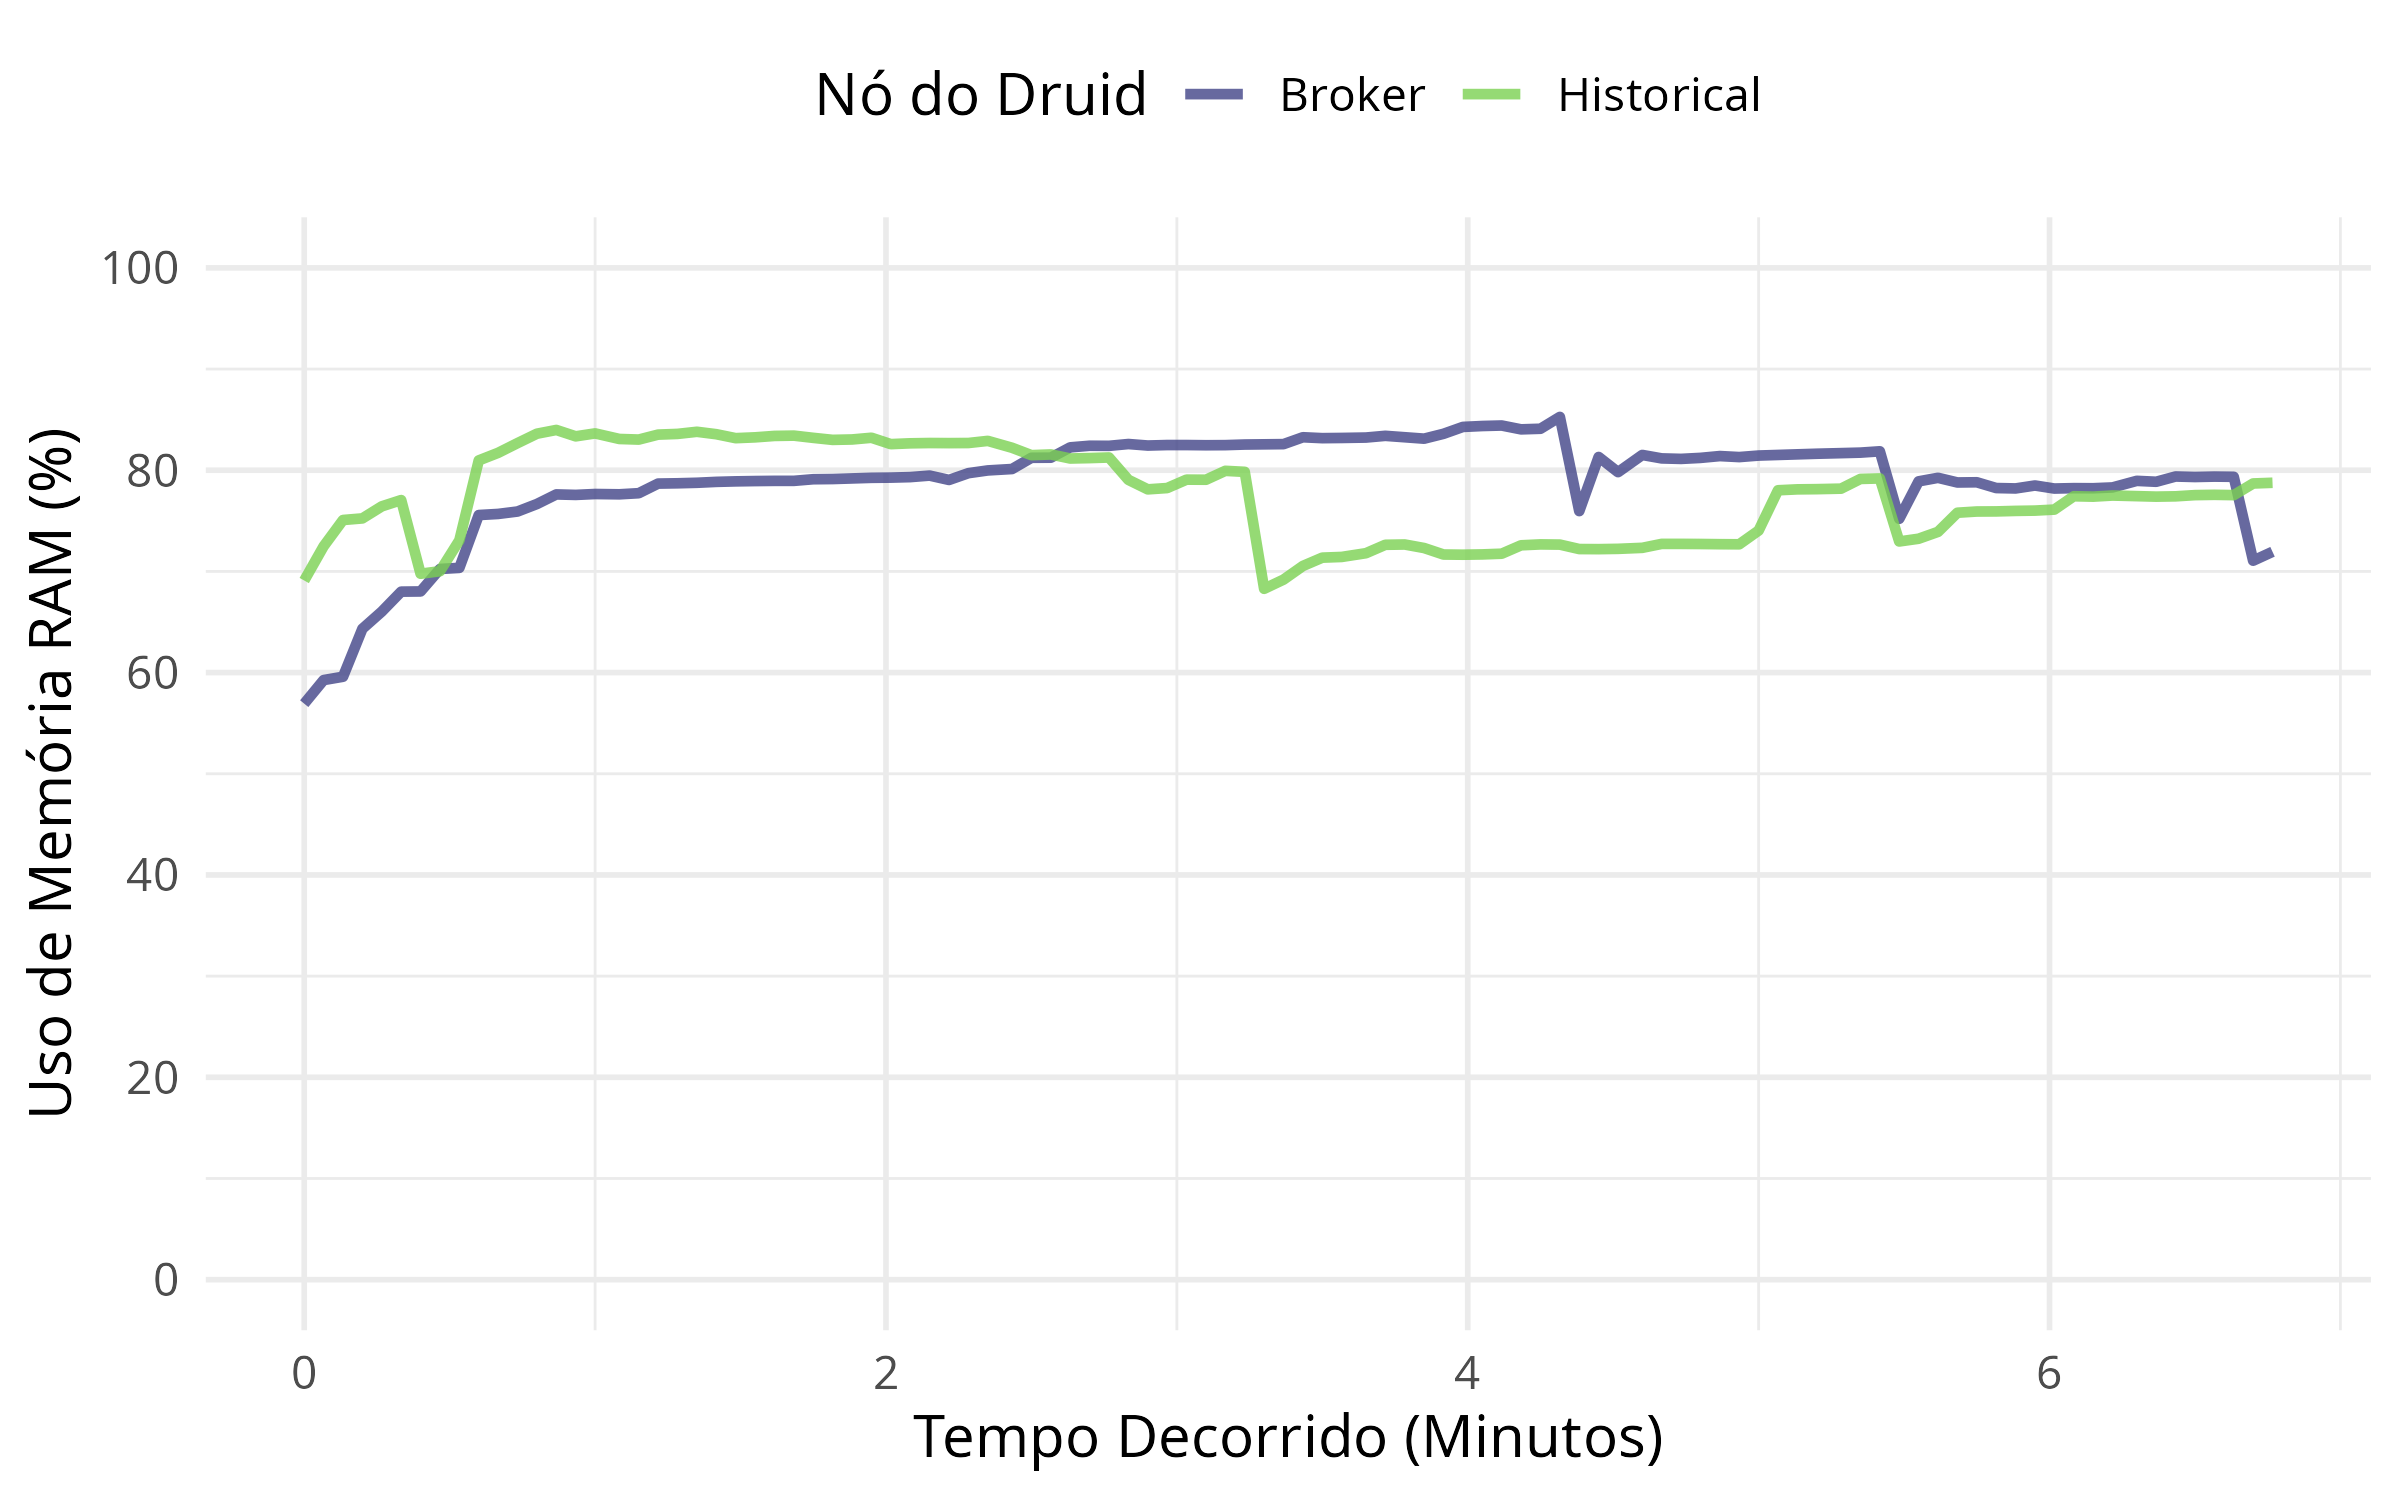
\includegraphics[width=0.8\textwidth]{analise_R/plots/ram_usage_new.png}
    \caption{Oscilação do Consumo de RAM no Apache Druid.}
    \label{fig:ram_usage}
\end{figure}

\subsection{Análise Operacional do Cenário de Crise Ambiental (2025)}

Após a otimização arquitetural, a plataforma foi submetida a um cenário extremo de estiagem e incêndios florestais baseados no monitoramento de anomalias térmicas via sensoriamento remoto \cite{giglio_modis_2016}. O sistema permitiu transformar o volume massivo de biometria de calor crua (\textit{raw fire points}) em inteligência tática aplicável à infraestrutura nacional.

\subsubsection{Panorama Geral e Dinâmica nos Biomas}

A crise ambiental atingiu o território nacional de forma aguda e irregular. A Figura \ref{fig:dashboard_outubro} ilustra um painel analítico focado na amostra de outubro de 2025 (pico da estiagem), evidenciando os focos ativos, a área destruída e a severidade do evento (FRP). O painel atesta a macro-evolução do desastre, marcada por um comportamento escalonado e contínuo impulsionado pelo acúmulo agudo das condições de seca.

\begin{figure}[H]
    \centering
    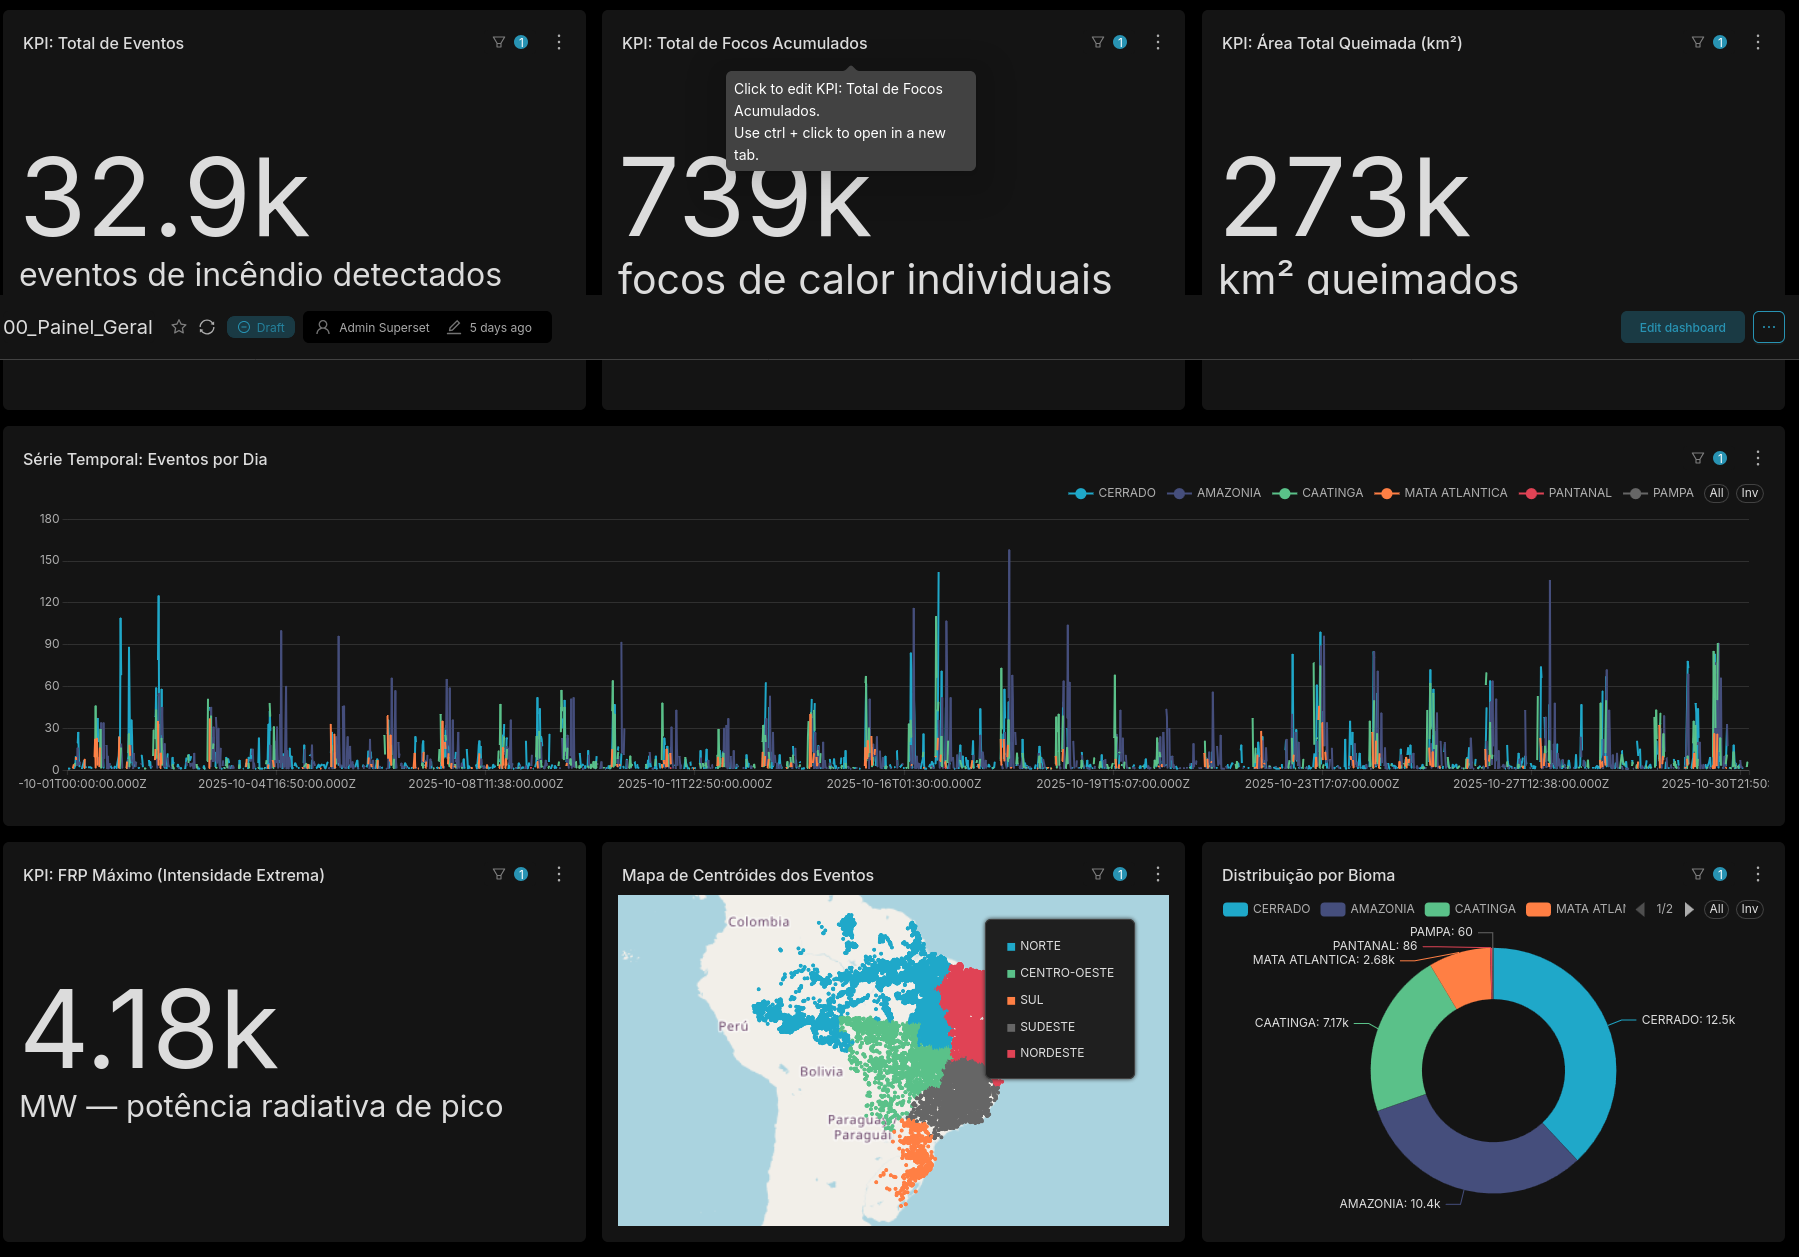
\includegraphics[width=0.9\textwidth]{materiais_apoio/figures/DashBoard.png}
    \caption{Visualização Analítica de Ignições (Apache Superset).}
    \label{fig:dashboard_outubro}
\end{figure}

\subsubsection{Impacto em Comunidades Vulneráveis: Terras Indígenas}

Uma das principais premissas táticas foi mensurar o nível de ameaça sistêmica às comunidades originárias utilizando as malhas poligonais oficiais da FUNAI. O motor analítico rastreou com precisão o cruzamento físico e a aproximação marginal (buffers) das coordenadas de fogo sobre essas demarcações. O resultado prático consolidou um ranking geoespacial de pressão social exibido na Figura \ref{fig:ranking_tis}, revelando os territórios indígenas que apresentaram alta vulnerabilidade espacial.

\begin{figure}[H]
    \centering
    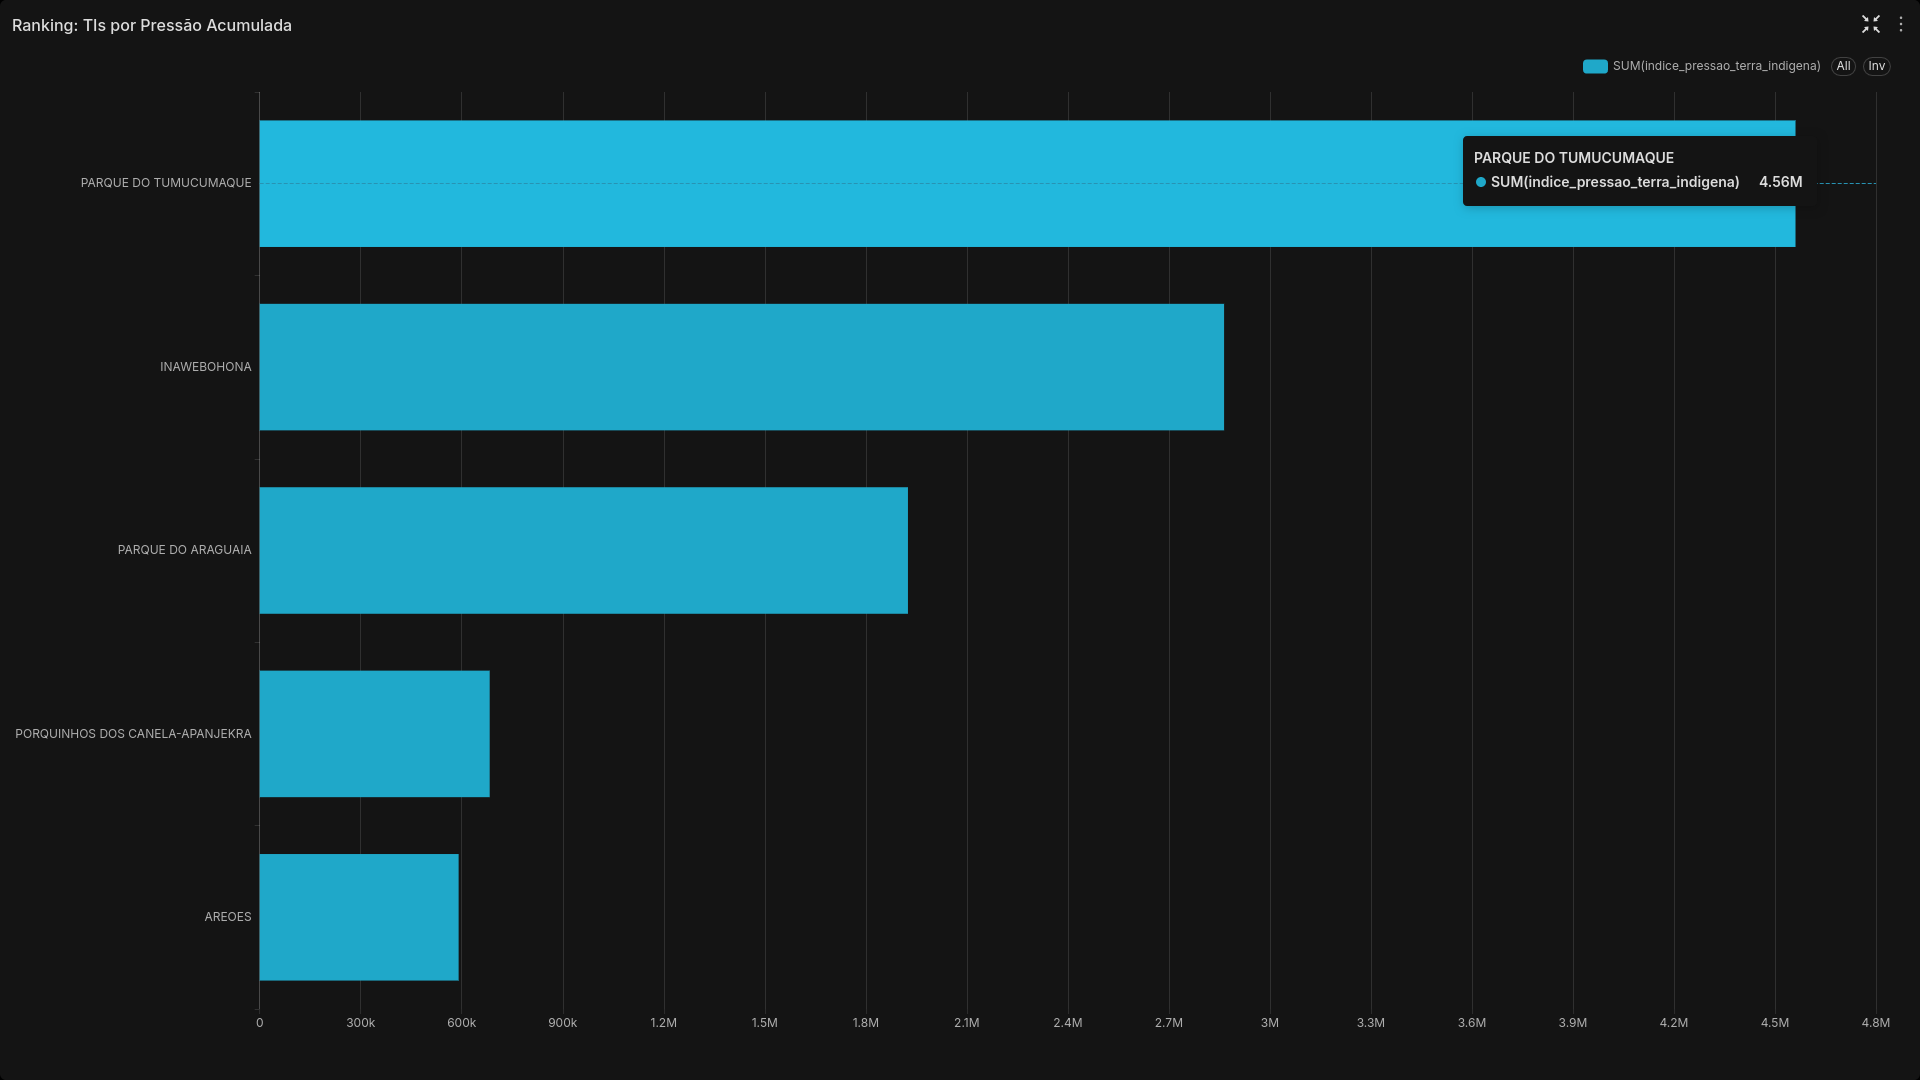
\includegraphics[width=0.9\textwidth]{materiais_apoio/figures/PressãoIndigena.png}
    \caption{Volumetria de Focos em Terras Indígenas.}
    \label{fig:ranking_tis}
\end{figure}

A agregação analítica classificou a \textbf{Terra Indígena Parque do Araguaia} (Formoso do Araguaia/TO) no 3º lugar do ranking de vulnerabilidade com base nos dados de 2025. Levanta-se a hipótese de que essa elevada concentração de anomalias térmicas reflita o avanço do pólo agroindustrial para a porção sul da Ilha do Bananal. Embora o índice calculado não determine causalidade direta para eventos isolados, as métricas parecem corroborar a narrativa cíclica de degradação na região. Segundo reportagem do portal G1, em setembro de 2026, um novo incêndio destruiu 38 residências na Aldeia Canoanã, inserida na mesma demarcação \cite{g1_canoana_2026}. A identificação prévia deste território no topo do ranking sugere que a plataforma pode atuar como um instrumento de apoio para o mapeamento de tendências de exposição e subsidiar ações preventivas.

\subsubsection{Ameaça à Infraestrutura Crítica: Setor Elétrico e Saúde (SUS)}

A integração central do projeto foi materializada na intersecção veloz entre as medições dos satélites termais e a infraestrutura civil mapeada. Centros hospitalares localizados nos arredores dos epicentros rurais de incêndio sofreram o reflexo primário de densas massas regionais de fumaça, gerando alto impacto na região de cobertura das unidades de saúde. O controle exibido na Figura \ref{fig:hospitais_criticos} rastreou não apenas o quantitativo, mas a intensidade da radiação (FRP) sobrepostas às coordenadas do Cadastro Nacional de Estabelecimentos de Saúde (CNES).

\begin{figure}[H]
    \centering
    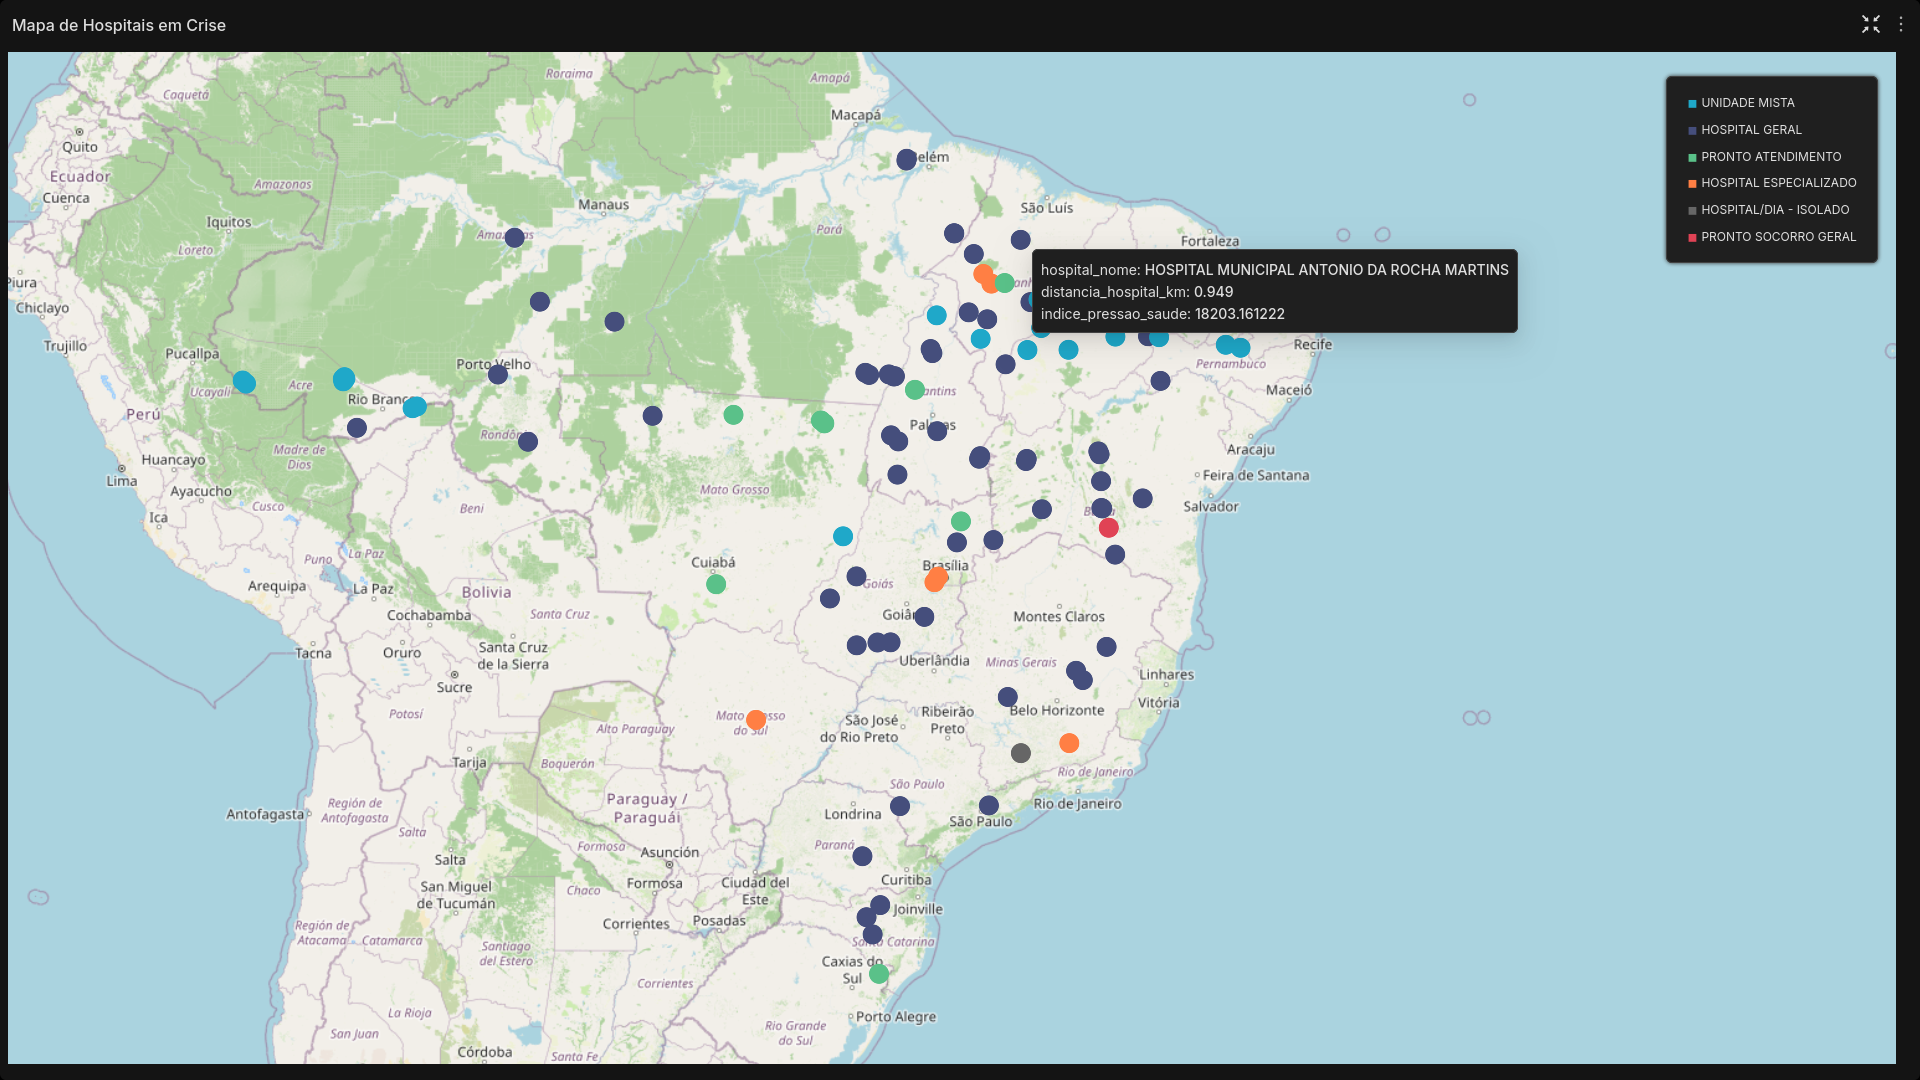
\includegraphics[width=0.9\textwidth]{materiais_apoio/figures/HospitaisCriticos.png}
    \caption{Monitoramento de Hospitais Expostos ao Fogo.}
    \label{fig:hospitais_criticos}
\end{figure}

Da mesma forma sistêmica, os dados estenderam o cordão sanitário para resguardar a malha operada pelo Operador Nacional do Sistema Elétrico (ONS). A exposição das linhas de transmissão a focos de calor intenso gera o perigo extremo de arcos elétricos e curtos-circuitos da rede neutra para a terra (desligamento forçado). 

A Figura \ref{fig:evolucao_energia} modela a progressão sistêmica dessa ameaça ao longo de todo o ano de 2025. A série temporal atua como uma evidência analítica crucial para demonstrar a assimetria da crise: o índice permanece baixo no primeiro semestre e cresce de forma acentuada a partir de setembro e outubro nas regiões de escoamento energético. Essa métrica expõe como as condições de seca extrema submetem repentinamente a infraestrutura a um aumento de pressão crítico e de complexa mitigação logística.

\begin{figure}[H]
    \centering
    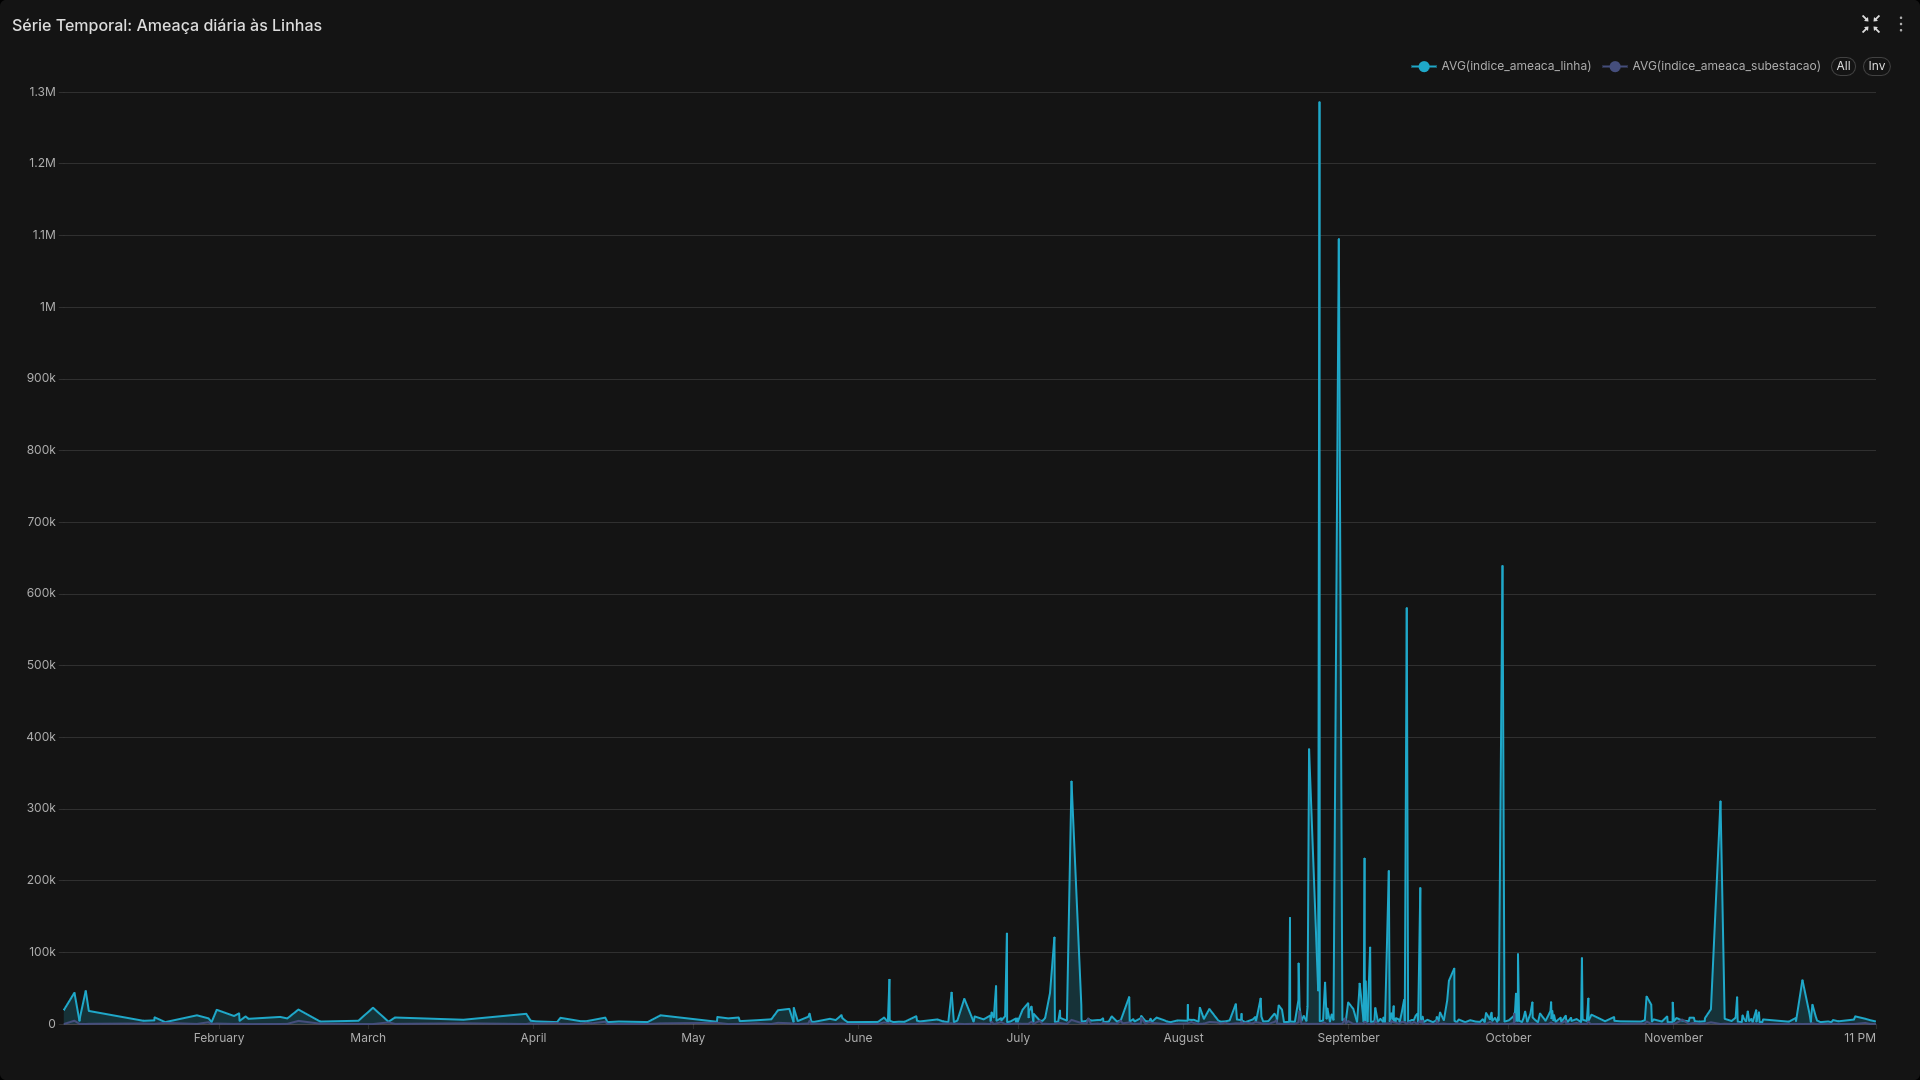
\includegraphics[width=0.9\textwidth]{materiais_apoio/figures/EvoluçãoDaPressãoEletricaAolongodoAno.png}
    \caption{Evolução da Ameaça à Infraestrutura Elétrica (ONS).}
    \label{fig:evolucao_energia}
\end{figure}

Aliando o risco termal agudo com as métricas topológicas (\textit{Betweenness Centrality}) previamente estabelecidas, a plataforma consolidou a Tabela \ref{tab:subestacoes_ameacadas}. Ela enumera as subestações mais expostas a interrupções operacionais, ordenadas pelo potencial de indução de risco sistêmico em rede. O cruzamento destacou vértices infraestruturais vitais, a exemplo da SE Rio Verde Norte (GO), elo de escoamento do Norte para o Sudeste; da SE Assis (SP), coletora da bacia do Rio Paraná; e da SE Trindade (GO), pivô na interligação Norte-Sul \cite{epe_pde_2032, ons_mapa_2026}.

Quando nós de energia sob Risco \textbf{Extremo} sofrem desligamento forçado, a matriz energética redistribui a carga base por rotas mais longas. Esse fenômeno sobrecarrega linhas secundárias e aciona sistemas primários de proteção (como o Esquema Regional de Alívio de Carga - ERAC), culminando no risco agudo de apagões regionais e blecautes em cascata por todo o subsistema interligado do país \cite{ons_procedimentos_2026}.

\begin{table}[H]
\centering
\caption{Top 10 Subestações Críticas via Betweenness Centrality.}
\label{tab:subestacoes_ameacadas}
\resizebox{\textwidth}{!}{%
\begin{tabular}{lrrc}
\toprule
\textbf{Subestação} & \textbf{Capacidade (MW)} & \textbf{Betweenness Centrality} & \textbf{Risco Cascata} \\
\midrule
R.VERDE NORTE & 1344.00 & 100.00 & EXTREMO \\
ASSIS & 2808.00 & 98.21 & EXTREMO \\
TRINDADE & 1600.00 & 91.33 & EXTREMO \\
SAMAMBAIA & 6000.00 & 89.30 & EXTREMO \\
XAVANTES & 600.00 & 89.22 & EXTREMO \\
BANDEIRANTES & 2542.00 & 87.68 & EXTREMO \\
LONDRINA ESU & 2016.00 & 59.42 & ALTO \\
BOM.JES.LAPA II & 850.00 & 47.07 & MEDIO \\
LUZIANIA & 450.00 & 46.83 & MEDIO \\
MIRACEMA & 10359.00 & 45.51 & MEDIO \\
\bottomrule
\end{tabular}%
}
\end{table}


